% title and thanks
%TC:ignore 
\begin{titlepage}
\begin{center}

\textsc{\LARGE University of Manchester}\\[1.5cm]
\textsc{\Large School of Computer Science\\Project Report 2014}\\[0.5cm]

% Title
\HRule \\[0.4cm]
{ \huge \bfseries Using Machine Learning to predict personal expenditure \\[0.4cm] }
\question{I'm still not sure on the title, the report includes: prediction, historical finances and security}
\HRule \\[1.5cm]

% Author and supervisor
\begin{minipage}{0.4\textwidth}
\begin{flushleft} \large
\emph{Author:}\\
Pez \textsc{Cuckow}
\end{flushleft}
\end{minipage}
\begin{minipage}{0.4\textwidth}
\begin{flushright} \large
\emph{Supervisor:} \\
Dr Gavin \textsc{Brown}
\end{flushright}
\end{minipage}

\vfill

% Bottom of the page
%{\large \today}

\end{center}
\end{titlepage}
%TC:ignore
\begin{abstract}
A complete understanding of personal finances is becoming increasingly important as the average persons disposable income has decreased due to a changing financial climate.

The aim of this project is build to an application that makes it easier to manage a users personal finances. This is split into two halves, accessing historical information in an easy to understand way and using machine learning techniques to predict future financial information \todo{Still needs adjusting}. The security considerations of storing personal finance information is also considered.

This begins with a review of the existing commercial personal finance applications and the current techniques used to forecast time-boxed financial data, such as the value of a stock on the stock market, before detailing the design and implementation of the application.

Having completed the application, the performance the selected techniques are outlined, before discussing possible extensions to the application to improve it's accuracy and increase it's feature set and possible further research. \todo{This needs adjusting}
\\
\par\noindent{\textbf{Project Title}: Using Machine Learning to Predict Personal Expenditure \\
\textbf{Author}: Pez Cuckow \\
\textbf{Degree}: Computer Science with Business and Management \\
\textbf{Supervisor}: Dr Gavin Brown} \\

\par\noindent{\small{\bf Keywords:} Markov Chain Models, Weighted Arithmetic Mean, Responsive Web Design, Web System Security}

\end{abstract}
%TC:endignore

%TC:endignore 
%\clearpage
\vspace*{1.4in}
\begin{center}
  {\textbf{Acknowledgements}} \\
\end{center}
\begin{quotation}
  Thanks everyone, y'all great.
\end{quotation}

% define words
\newglossaryentry{transactor}
{
  name={transactor},
  description={somewhere money is spent, e.g. Tesco, Sainsbury's, Byte Cafe.}
}

\newglossaryentry{transaction}
{
  name={transaction},
  description={a single movement of money from/to a Transactor}
}

\newglossaryentry{category}
{
  name={category},
  description={transactors have a category and a subcategory, e.g. Tesco = Shopping, Groceries}
}

\newglossaryentry{reference}
{
  name={reference},
  description={the memo or message that is included on the bank statement with a transaction}
}

\newglossaryentry{mapping}
{
  name={mapping},
  description={this connects the reference found on a statement to a Transactor. e.g. Snbs, Sains => Sainsbury's}
}

\newglossaryentry{globaltransactor}
{
  name={global transactor},
  description={the system holds two collections of transactors and mapping's, the global ones
are shared between all users, and only accessed with the admin panel.}
}

\newglossaryentry{usertransactor}
{
  name={user transactor},
  description={unique to each user}
}

% start of document
\tableofcontents
\listoffigures
\listoftables
\printglossaries

\clearpage

% Password entropy & security
% Personalised model from Five models detail, per catecory, per person
% Hypothesise one models

% start of writing
\begin{comment}
This chapter puts the work into context. Having read it, the reader should be left in no doubt as to:

- the topic area to which the work applies
- why the work is being done
- what else has been done in the area and by whom
 - how the author proposes to tackle the problem: The project proposal is often expressed in terms of a main objective and possibly one or more additional objectives. It is useful to define "milestones" or "sub-goals" that mark the progress towards the objectives. 
 - It is common to end this chapter with a brief overview of each of the subsequent chapters of the report.
 
\end{comment}

\chapter{Introduction}
\label{cha:introduction}
Traditionally the management of personal finances is performed by viewing bank statements provided by the users bank. In the modern age of `Internet banking', banks offer a limited set of tools that mimic the paper statements seen historically.

This project sets out to build an online application that can be used to manage personal finances. There are two main parts of the project; firstly users can upload bank statements, which are displayed and navigated in an intuitive manner; secondly, once the application has enough historical data, predicting the users future outflow.

\section{Motivation}
There are four main steps when producing and using a budget: recording previous expenses, sorting these into categories, using this historical information to estimate future expenditure, and evaluating the accuracy of predictions based on the new information and adjusting accordingly.

Since the liquidity crisis of 2009 \parencite{gore2010}, budgets have been squeezed and the average personal disposable income has fallen significantly, hitting a nine-year low in 2012 \parencite{barnard2012households}. Experts suggest that ``Budgets are essential for financial planning'' \parencite{wsj2013budget}, research suggesting that personal budgets lead to a ``positive impact'' on ``mental wellbeing'' \parencite{tlap2013budget} and guides from UCAS, the UoM SU Advice Centre and The Manchester University Crucial Guide encouraging use of budgeting, it is clear that producing a budget is of benefit.

In an informal survey\footnote{Appendix \ref{app:budgetsurvey}} by the researchers, however, the majority of students questioned did not heed this advice, and were not following a budget. Producing an easier way to manage personal finances and predict future outflow can hopefully reduce the barriers to entry for creating budgets and increase the people using one.

Increasing use of debit cards \parencite{bbc2010debit} means that bank statements contain more and more information about where people spend their money. With access to those bank statements now provided online, and most UK banks offering the option to export \gls{transaction} history, individual users can collate a database of their personal spending habits.

The increasing availability of this data, combined with more detailed \gls{transaction} history makes it potentially possible to automate the four main steps of producing a budget, and this is the main objective of the project.

\section{Aims and Objectives}
%\plan{Things I set out to do, designed by talking to people to get an idea of features they would like}
The key objectives of this project can be split into three parts, the management of statements, making predictions of future outflow using those statements and ensuring a high level of security.

\subsection{Statement Management}
Implement an intuitive way to view and manage personal finances.
%
There are several key parts to this, upload and parsing of \glspl{transaction} from statements downloaded from the users bank, resolving the \glspl{reference} found on the statement to the real world business they represent and categorising the individual \glspl{transaction} to make them easier to understand.
    
\subsection{Prediction}
Accurately predicting a users future \glspl{transaction} based on their \glspl{transaction} history.
%
The prediction should be made using a model that is fitted to each users individual spending patterns, and is evaluated in order to improve the model.
%
The application will need to predict whether or not spending will occur and how much money will be spent.

\subsection{Security}
The project should be secure and uphold the high security expectations of users uploading their personal information.
%
The application will deal with information of a sensitive nature, therefore strong security techniques are of high importance to ensure no loss of personally identifiable information. 
% 
The project should take this into account, considering possible attack vectors and taking steps to mitigate those attacks.

\section{Overview of Report}
\plan{This report covers some of the key design decisions, implementation decisions and then what the application does}

Chapter \ref{cha:background} reviews existing commercial personal finance applications and existing techniques used to forcast time-boxed financial information.

Chapter \ref{cha:design} details the key design decisions made when planning the software and how the techniques in the background research are applied.

Chapter \ref{cha:implementation} includes implementation specifics of some of the features outlined in the design, focused particularly on features that were difficult to implement.

Chapter \ref{cha:results} gives an outlined of the finished applications features through the use of screenshots in a walkthrough.

Chapter \ref{cha:testing} reviews the performance of the application in terms of prediction accuracy and user experience. \todo{Does it?}

The report concludes in chapter \ref{cha:conclusions} which compares the project aims to what was achieved, suggests further enhancements that could be added to the application and outlines some further research areas.

\todo{This needs to be completed}
\chapter{Background}
\label{cha:background}

\begin{comment}
Chapter 2: Background and literature survey
This chapter should give essential background information with references to published material in research papers, books, URLs, magazine articles and even newspapers. Expand on any references to other work that have been mentioned in Chapter 1. Refer to the notes on references (below) for the preferred way of referencing publications. The reader, stimulated by the presentation of ideas in this section, may be led to consult some or all of the referenced publications. This section will be useful for any student in a subsequent year who wishes to take the project further.
\end{comment}

As outlined in Chapter \ref{cha:introduction} the project consists of two major parts: a financial management service, which can be used to view historical spending and gain understanding of personal finances; and a forecasting element which predicts how much spending will occur in the future. 
\question{Include this?} \question{Technically it's spending or receiving "transaction" but this becomes very wordy?}

\section{Statement Management}
There are existing applications that implement similar features to the money management aims of this project\question{Mention the current "bad" internet banking here?}, most notably Lloyds TSB Money Manager, the first and only personal money management application provided by a UK bank and Mint.com a United States (US) only personal finance service \parencite{lloyds2014moneymanager, mint2014whatismint}.

\subsection{Lloyds Money Manager}
The service is available to Lloyds TSB current account holders as part of their online banking and it's features revolve around documenting historical spending \parencite{lloyds2014money}.

The key features include:
\begin{itemize}
\item Categorising spending
\item Creating spending plans per category
%\item View dates money came in and out in a calendar
\item Viewing money spent per category
\item Track progress of budget targets
\end{itemize}

Customer reviews of the service highlight the usefulness of spending analysis screen, which includes a breakdown of spending in each \gls{category} (Fig. \ref{fig:moneymanager}, as well as the spending calendar, which displays money spent in a day by day format.
%
The reviews, however, also highlight some shortcomings, noting that changes to categories are not reflected immediately, categories are often incorrect and that it's not possible to override the \gls{category} for a single transaction, for example food bought at a petrol station is placed in the Car \gls{category} and cannot be moved \cite{moneywatch2011lloyds, moneysupermarket2011lloyds}.

\begin{figure}[h]
    \centering
    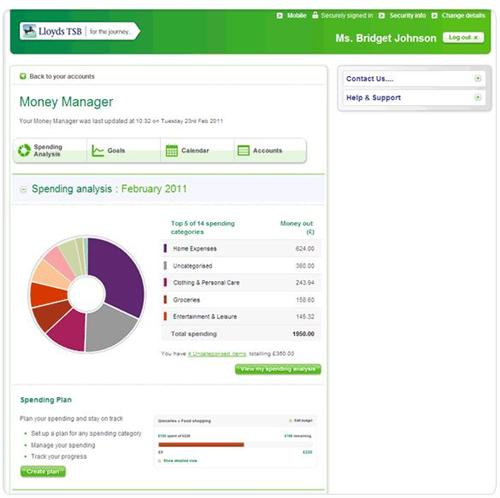
\includegraphics{background/moneymanagerchart}
    \caption{Spending Analysis by category on Money Manager \parencite{lloyds2014money}}
    \label{fig:moneymanager}
\end{figure}

A key advantage of the money manager is that Lloyds already have access to their customer data, so there is no data entry or upload required, which could be confusing and off-putting to potential users.

\subsection{Mint.com}
Mint.com offers very similar features to LLoyds but it limited to the US. However, Mint automatically logs into the users online bank account and downloads their statements authenticating with their banking username and password. It's reported that this feature relies on the use of application programming interface's (API) at each bank which Intuit (the company behind Mint) have negotiated access individually, though Intuit have published no information to support or dispute this \cite{stackoverflow2012bankingapi, stackoverflow2012bankingapi2}.
% 
Although this feature is clearly useful and saves time for the users, it does make Mint responsible for storing their customers Internet banking passwords and presumably involves fee payments to the banks providing these API's. \question{Should I have more detail on what mint/lloyds do?}
%
For these reasons it was decided that automatic statement uploading was outside of the budget and scope of this project, however, the project should support manual upload of statements to avoid date entry of users. \question{Does this need backing up?}

\subsection{Mobile Apps}
Mobile applications or `apps' as they are commonly known have seen a surge in popularity since the release of startphones and are a common target for small pieces of software, such as financial organisation \parencite{purcell2011half}.

The three most popular iPhone personal financial applications \cite{itunes2013topapps}, at the time of planning the project, all offered features very similar to those found in the Lloyds Money Manager and Mint. The most popular features being grouping money by \gls{category} and graphs of spending history.
% 
However, they all had the same drawback, the user had to manually enter all of their transactions and set categories for them, which appears time consuming and error prone, particularly on a mobile app \cite{spendee2014spendee,budgt2013budgt,bluetags2014pocket}.

The increase of mobile usage should be considered when planning the features of the project, with the project ensuring mobile compatibility and if possible, avoiding manual data entry. \plan{This needs improving}

\section{Prediction}
%\plan{Ways other people try to predict the future expenditure (in stocks etc...)}

There are various approaches to making predictions of financial spending, each with their own advantages and disadvantages \question{Not sure if this is relevant}. Predicting future transactions before they occur is technically similar to the work done by investors on the stock market, where the objective is to predict whether the value of a stock will fall or increase in order to make buy/sell decisions.

Preifer and Carraway demonstrated that Markov Chain Models can be used to model customer relationships with a business and predict the expected value of a marketing engagement with an individual customer. By creating a transition matrix of a particular customer transitioning from not spending to spending and visa versa over five periods\footnote{An `illustration' assuming a customer will never return after 5 months of not spending}, they were able to estimate the likely-hood of a spend occurring in a given period, Fig. \ref{fig:preifermarkovchain} shows a graphical representation of the model that was produced, the states represent the five periods, where $p_{i}$ is the probability of the transition occurring during period $i$ \cite{pfeifer2000modeling}.
% 
The paper is able to calculate the expected loan to value ratio (LTV) for the customer over the periods, by taking a matrix costs and gains associated with a purchase in each period and multiplying that by the probability of a purchase occurring taken from the transition matrix. This gives the expected present value for each period, which can be used to decide when to end a relationship with a customer (preventing the costs).
%
They demonstrate applying Markov Chain Models to a larger dataset, calculating the optimal policy for ending relationships with customers depending on varying costs concluding that the use of MCM's is an effective way of making customer relationship decisions. However, this paper assumes the company performing these predictions already knows how much money a customer will spent during each interactions and is focussed around calculating the probability of a spend occurring. An implementation applied to the personal spending space will require a way to predict the value of the future transaction.
\question{Mention what HMM's are here?}

\begin{figure}[h]
    \centering
    %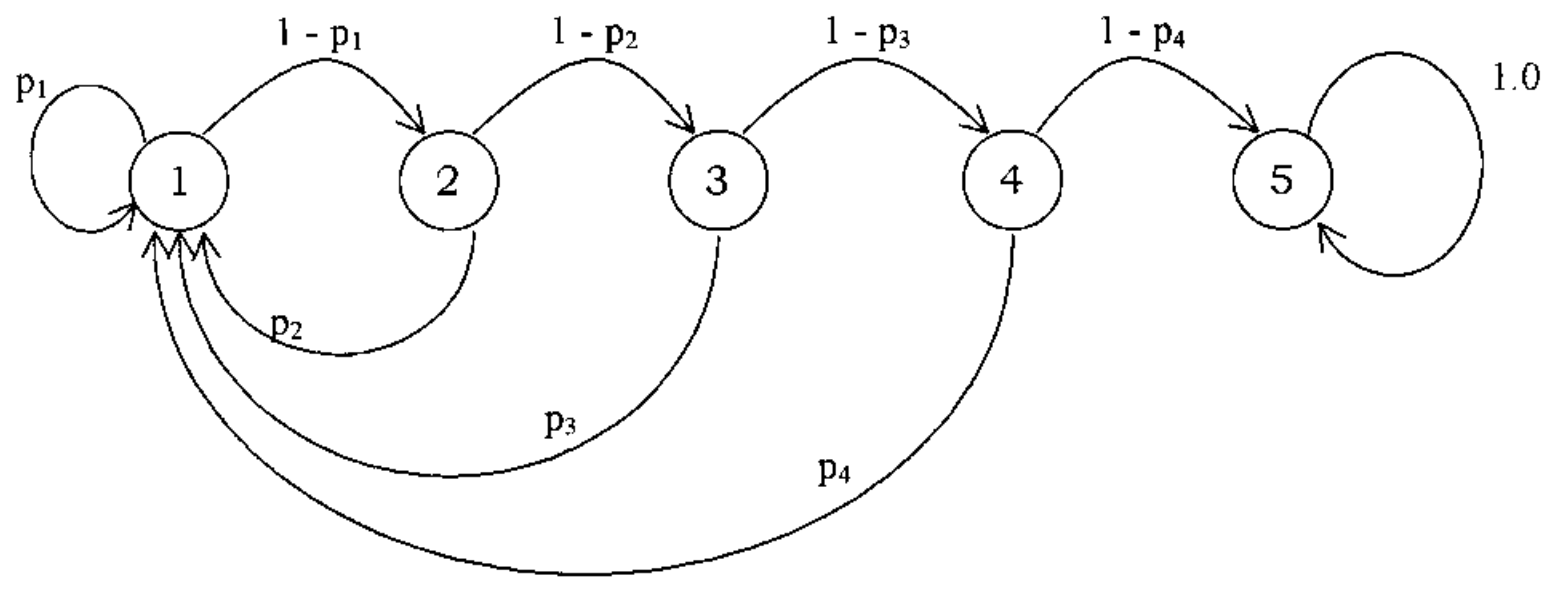
\includegraphics[width=\textwidth]{background/markovchain}
    \begin{tikzpicture}[start chain=going right]
    \node[state, on chain]                 (1) {1};
    \node[state, on chain]                 (2) {2};
    \node[state, on chain]                 (3) {3};
    \node[state, on chain]                 (4) {4};
    \node[state, on chain]                 (5) {5};
    \
    \draw[
        >=latex,
    %   every node/.style={above,midway},% either
        auto=right,                      % or
        loop above/.style={out=75,in=105,loop},
        every loop,
        ]
     (1) 	edge[bend left] node [above]{$1 - p_{1}$}   (2)
      		edge[out=145,in=220,loop,looseness=6]             node {$p_{1}$}   (1)
     (2) 	edge[bend left] node[above]{$1 - p_{2}$}   (3)
      		edge[bend left=90,,in=120]             node {$p_{2}$}   (1)
     (3) 	edge[bend left] node[above] {$1 - p_{2}$}   (4)
     		edge[bend left=90,in=105,]             node {$p_{3}$}   (1)
     (4) 	edge[bend left] node [above]{$1 - p_{2}$}   (5)
     		edge[bend left=90,in=90]             node {$p_{4}$}   (1)
     (5) 	edge[out=40, in=320,loop,looseness=6] node[right]{$1.0$}   (5);
    
    
    % The \draw path is like the one above.
    \end{tikzpicture}
    \caption[Markov Chain Model of customer spending]{Markov Chain Model for a particular customer over five periods \parencite[Adapted from Fig. 1]{pfeifer2000modeling}}
    \label{fig:preifermarkovchain}
\end{figure}

% OTHER PREDICTION
Research by Singh et al., from the Massachusetts Institute of Technology, studied the spending behaviour of 52 adults and investigated the impact of social interactions, including text messages, phone calls and face-to-face meetings, on the participants spending in order to predict their spending behaviour. Using a Na\"{i}ve Bayes classifier and selecting a subset of their available features using an Information Gain approach, choosing those with most relevance to each classification task, they were able to correctly classify whether the participant would overspend, explore a diverse range of businesses and remain loyal to a business with 72\% overall accuracy. They concluded that social factors, were better ``predictors of spending behaviour'' than personality traits, which had been previously studied \parencite{singh2013spendingbehaviour}.
%
Although this paper did not study the affects of the participants previous transactions on spending, they were able to predict the users spending behaviour, highlighting that factors other than the transaction history may be of importance when trying to predict a users future outflow. However, the paper does not attempt to make a prediction of the amount spent or how many transactions occur.

% AVERAGES
Smoothing is typically applied to financial market data, for example the value of a particular stock on the FTSE 100. The most common techniques are simple, weighted and exponential moving averages, which all reduce the noise found in the data potentially revealing an orderly process, by removing outliers found in the data. The result of this effect can be seen in Fig \ref{fig:dashweightedaverages} \parencite{dash2012movingaverages}.

\begin{figure}[h]
    \centering
    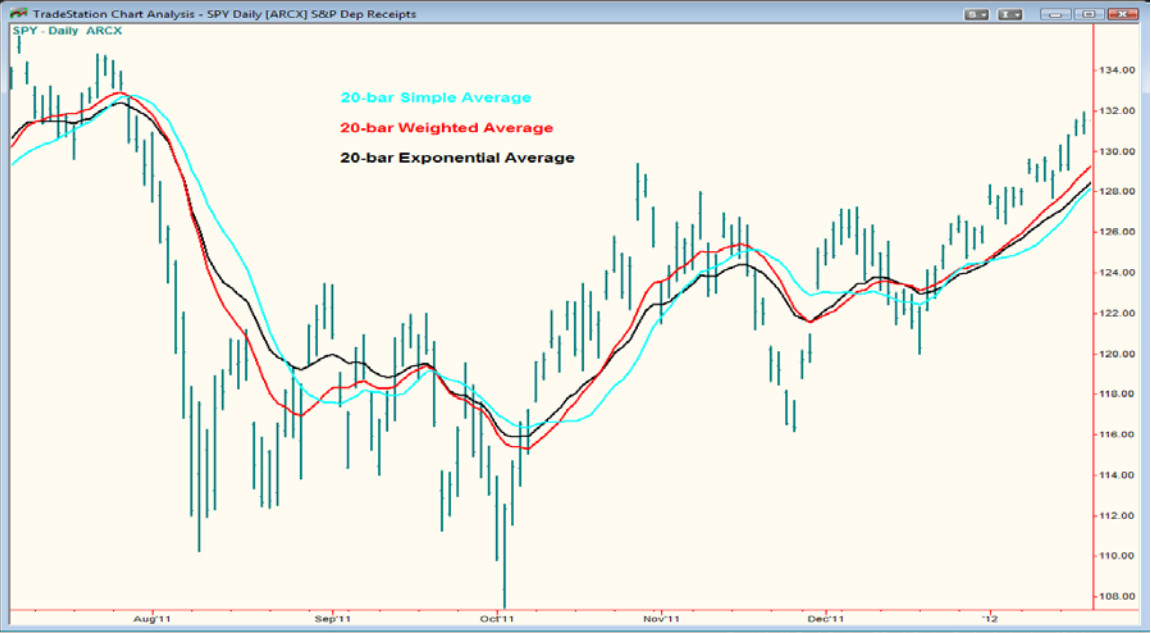
\includegraphics[width=\textwidth]{background/movingaverages}
    \caption[SMA, WMA and EMA of the S\&P500]{Simple Moving Average (MA) [blue], Weighted MA [red] and Exponential MA [black] of the S\&P500 \protect\footnotemark \parencite[Fig. 5]{dash2012movingaverages}}
    \label{fig:dashweightedaverages}
\end{figure}
\footnotetext{A stock market index of 500 American companies, the US equivalent of the FTSE 500}

These techniques can be applied to a discrete set of numerical time series data, such as personal expenditure over time in order to make an estimate of what the next value in the series will be \parencite{filliben2003nist}. A prediction can be made using the formula in Fig. \ref{fig:weightedmeanforumla}, where $w_{i}$ is the weight and $x_i$ is the value at time period $i$. Simple smoothing is the equivalent of $w_i = 1$, while exponential smoothing is based around a negative exponential law such as $w_i = e^{-n+i}$, both are examples of weighted smoothing and the weights can be decided in different ways depending on what is being predicted. Time periods with a higher weight have a greater affect on the mean, so in order to make a future prediction, the most recent time period would have a higher weight. \question{The chosen implementation details in the design section}

\begin{figure}[h]
    \centering
    \[
        \frac{w_1 x_1 + w_2 x_2 + \cdots + w_n x_n}{w_1 + w_2 + \cdots + w_n}.
    \]
    \caption{Using weighted smoothing to predict a future value}
    \label{fig:weightedmeanforumla}
\end{figure}

% Holt winters extends smoothing, to take into account trends in data
Smoothing (and therefore prediction) can be extended to take into account trends and possible seasonal fluctuations using double and triple smoothing, respectively. A technique known as `Holt-Winters double exponential smoothing` takes into account trends in data, which single smoothing does perform accurately with, by factoring the weighted average growth between previous the time series when calculating the average for each period \parencite{kalekar2004holtwinters}. \question{A demonstration of this is in chapter X?}
% 
Extending the calculation into double and triple smoothing when estimating a users future outflow was decided as a possible extension for the project. \question{Where to mention this?} 

\section{Security}
\question{Should I mention the password entropy paper here? Currently in design}



\begin{comment}
Chapter 3: Design
This chapter starts to describe the student's own work. It is where the main design aspects of the project are described. The style of presentation may reflect the life cycle of the project, for example commencing with the Requirements Analysis, but it should not read like a diary. The design should be clearly and precisely described with supporting diagrams. The presentation should be at a fairly high level without excessive detail. This chapter is a suitable place to justify your choice of architecture, implementation technologies and APIs used.
\end{comment}

\chapter{Design}
\label{cha:design}
This chapter covers design of the system, including an overview of the architecture and descriptions of the key components. 

\section{Statement Management}
The statement management features of the application were selected based on the functionality observed during the background research and conversations with potential users, asking what features they enjoyed from their current Internet banking and what additional features they would find useful to manage their statements

The key features include; parsing of files downloaded from Internet banking, mapping transactions found in the files to real world businesses (transactors), organising transaction history by \gls{category} or transactor and viewing all transactions at a particular transactor.

\subsection{Upload} \label{subsection:upload}
To get a users transaction history they must first upload a file containing their historical transactions.

The major UK banks tested\footnote{Natwest, First Direct and HSBC} provided statement downloads in Quicken, Microsoft Money or Microsoft Excel format. Further investigation revealed that the underlying formats were Quicken Interchange Format (QIF), Open Financial Exchange (OFX) and comma-separated values (CSV).

As there is no pre-defined standard for bank statements in CSV format, upon investigation, it became clear that the banks used completely different structures. It was decided the application would parse the QIF and OFX formats, following their respective specifications. Examples of QIF and OFX can be seen in Fig. \ref{fig:qifofxformat}.

It was quickly identified that although the QIF/OFX files were following the same specification, depending on the bank they had different structures, and in some cases the structures even varied within the same bank, depending on the exact wording of the download. Interestingly an OFX file downloaded from First Direct was found to be in QIF format, despite an \lstinline$.ofx$ suffix.

Notably there were discrepancies with the formatting of dates in QIF. The specification from Intuit\footnote{The developers of Quicken and QIF} does not specify a date format \cite{quiken2010qif}. The sample files tested included dates in D-M-Y, M-D-Y and Y-M-D format.

\begin{figure}
\centering
\begin{lstlisting}
% QIF FORMAT
!Type:Bank
D28-06-13
PASDA SUPERSTORE    TROWBRIDGE
T-15.00
^
D28-06-13
PPAYPAL PAYMENT
T-12.50
^
\end{lstlisting}
\caption{Two transactions in QIF format}

\begin{lstlisting}
% OFX FORMAT
<STMTTRN>
<TRNTYPE>POS</TRNTYPE>
<DTPOSTED>20130628</DTPOSTED>
<TRNAMT>-15.00</TRNAMT>
<NAME>ASDA SUPERSTORE</NAME>
<MEMO>TROWBRIDGE</MEMO>
</STMTTRN>
<STMTTRN>
<TRNTYPE>DEBIT</TRNTYPE>
<DTPOSTED>20130618</DTPOSTED>
<TRNAMT>-12.50</TRNAMT>
<NAME>PAYPAL PAYMENT</NAME>
</STMTTRN>
\end{lstlisting}
\caption{Two transactions in OFX format}
%\label{QIF compared to OFX for two identical transactions}
\label{fig:qifofxformat}

\end{figure}

To combat this, three steps of resiliency were added to the design of the upload system, seen in Fig. \ref{fig:fileupload} \todo{Recompile this figure}.

\begin{figure}[h]
    \centering
    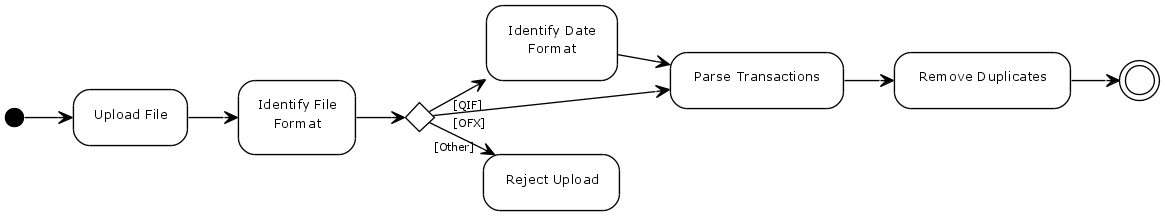
\includegraphics[width=\textwidth]{design/upload-activity}
    \caption{Activity diagram for statement uploads}
    \label{fig:fileupload}
    
    \begin{comment}
(start)->(Upload File)->(Identify File Format)-><a>[QIF]->(Identify Date Format)->(Parse Transactions),
<a>[OFX]->(Parse Transactions)->(Remove Duplicates)->(end),
<a>[Other]->(Reject Upload)
    \end{comment}
\end{figure}

Having uploaded the file the system first identifies the file type by looking inside the file and parsing its contents, ignoring the extension and rejecting the file if it matches neither format.

If the file is QIF the parser parses all transactions up front and evaluates the format of the dates. If the dates are found to have the format \lstinline$00-00-0000$ the system needs to decide whether that's DD-MM-YYYY or MM-DD-YYYY, otherwise performing standard date parsing of the string.
%(\lstinline$\d{1,2}[/-]\d{1,2}[/-]\d{2,4}$ in regular expression)
%
To decide between D-M-Y or M-D-Y the application goes through all the dates and attempts to parse in both formats, if a format fails it is marked as incorrect. This leaves the application in one of the four states, seen in Table \ref{table:datestates}. In the case of state 1 or 4 there is ambiguity and the application prompts the user. This ambiguity can be caused by dates that are malformed or a collection of dates falling within a range that doesn't have a day value over 12, as both formats parse correctly. 

\begin{table}[h]
\centering
\begin{tabular}{lll}
State & D-M-Y & M-D-Y \\
1     & true  & true  \\
2     & true  & false \\
3     & false & true  \\
4     & false & false
\end{tabular}
\caption{Possible states following evaluation of transaction dates}
\label{table:datestates}
\end{table}

In provisional user testing, it was discovered that users had a tendency to upload the same file more than once or to upload statements with an overlapping date range. To account for this, before creating a new \mbox{Transaction} the application checks for an identical transaction for the current user in the database and if one is found, skips creating a new Transaction. For speed this is done using a stored unique value, resulting from a SHA512 hash of date posted, transaction value, transactor, memo and transaction id\footnote{If a one was provided by the users bank}, which is generated when saving a Transaction to the database.

% 

\subsection{Named Entity Resolution}
Almost all functionality of the project relies on successfully mapping the text found on a bank statement that represents a business or person to a single entity in the application, known as a \gls{transactor} by the system. After a cleanup of different suffixes that banks append it was found that \glspl{transactor} are often referenced using several names.

Seen in Table \ref{tab:sainsburys}, Sainsbury's was referred to nine different ways in the statement data uploaded by the research participants and similar results are found for most \glspl{transactor}.

\begin{table}[h]
\centering
% SELECT name,count(t.id) as count FROM `transaction` AS t LEFT JOIN global_transactor_mapping AS g ON global_transactor_mapping_id = g.id WHERE global_transactor_mapping_id IN(SELECT id FROM global_transactor_mapping WHERE transactor_id = 7) GROUP BY global_transactor_mapping_id ORDER BY count DESC
\begin{tabular}{@{}ll@{}}
\toprule
Reference            & Occurrences \\ \midrule
sainsburys s/mkts    & 46          \\
sainsburys s/mkt     & 9           \\
sainsburys s/mkts cd & 7           \\
js online grocery    & 2           \\
sainsbury s/mkt cd   & 2           \\
sainsburys smkt      & 2           \\
js online grocer     & 1           \\
sainsburys superma   & 1           \\
sainsburys-superma   & 1           \\ \bottomrule
\end{tabular}
\caption{References to the entity `Sainsbury's' found in participant data}
\label{tab:sainsburys}
\end{table}

\subsubsection{Mapping to Entities}
In consideration of this, the concept of mappings was added to the system. A \gls{mapping} is a single \gls{reference} to a transactor, such as `sainsbury s/mkt'. A transactor has multiple mappings. Fig. \ref{fig:mapping} shows this structure.

\begin{figure}[h]
    \centering
    
\includegraphics[width=\textwidth]{design/simple-mappings}
    \caption{Overview of Mappings}
    \label{fig:mapping}
    
    \begin{comment}
%[User]-*<>[Transaction]
[Transaction]<>*-[TransactorMapping]
[TransactorMapping]<>*-[Transactor]
    \end{comment}
\end{figure}


\subsubsection{Global vs User}
As identified in the background research, it should be possible for users to both categorise and organise transactions according to their preferences and override existing categories, however categories chosen by a particular user should not affect other users. 

To support this the application stores two sets of mappings and transactions, \glslink{usertransactor}{User} and \glslink{globaltransactor}{Global}. The structure of the relevant objects is shown in Fig. \ref{fig:transactormappings}. A Transaction can have both a \glslink{usertransactor}{UserMapping} and a  \glslink{globaltransactor}{GlobalMapping}, in which case the UserMapping overrides the GlobalMapping when calling methods such as \inlinephp{getMapping()} on the Transaction.

\begin{figure}[h]
    \centering
    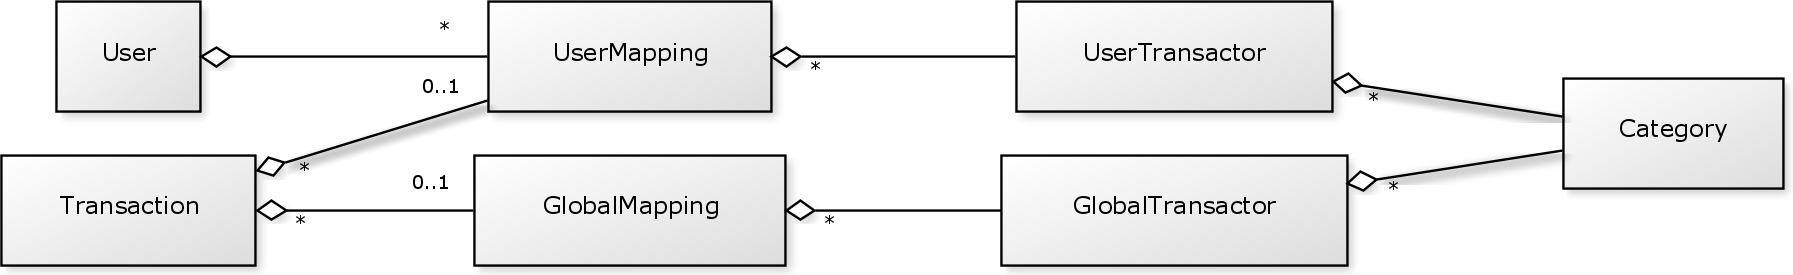
\includegraphics[width=\textwidth]{design/mappings}
    \caption{Overview of User Mappings}
    \label{fig:transactormappings}
    
    \begin{comment}
[Transaction]<>*-0..1[UserMapping]
[Transaction]<>*-0..1-[GlobalMapping]
[User]<>-*[UserMapping]
[UserMapping]<>*-[UserTransactor]
[UserTransactor]<>*-[Category]
[GlobalTransactor]<>*-[Category]
[GlobalMapping]<>*-[GlobalTransactor]
    \end{comment}
\end{figure}

\subsection{Suggestions}
Having mapped \glspl{reference} to entities, the system is able to use this knowledge to make suggestions of appropriate entities for unseen references in some cases to help streamline the naming process for potential users.
%
This is performed by taking the list of mappings and finding those with the smallest difference to the unseen reference. Difference can be calculated in several different ways, including the Levenshtein distance which calculates the number of single-character edits to transform between the two strings, implementation details for this project can be found in Section \ref{sec:suggestionimplementation} \parencite{levenshtein1966binary}.

\section{Prediction} \label{section:prediction-system}
In order to make a prediction of how much money a user will spend and receive in a given period, two steps need to be completed; predicting whether or not each individual transaction will occur in a given month; and estimating how much money will be involved.

Drawing from the research detailed in \autoref{cha:background}, the system uses a First-order Markov Chain model to decide whether or not transactions will occur, and weighted arithmetic means to predict how much money will be spent.

\subsection{Markov Chain Models}
% The probability of a transaction occurring can be calculated using Bayes' Theorem
% Probability of spend given that we didn't spend = probability of not spend given spend * probability of spend over probability of not spend.

An easy way to visualise the Markov Chain Models the system is creating is through a directed graph. Two frequent examples are shown in Fig. \ref{fig:transition-monthly} and \ref{fig:transition-one}, taken from participant data, where $0$ represents a transaction not occurring, $1$ is the opposite and the edges are labelled with the probability of transitioning from one to the other.

\begin{figure}[h]
\centering
\begin{tikzpicture}[start chain=going right]
\node[state, on chain]                 (0) {0};
\node[state, on chain]                 (1) {1};
\
\draw[
    >=latex,
    auto=right,                      % or
    loop above/.style={out=75,in=105,loop},
    every loop,
    ]
     (1) 	edge[loop above]    node {0.86}   (1)
      		edge[bend left]  node {0.14}   (0)
     (0)	edge[loop above]    node {0.8}   (0)
     		edge[bend left=40]  node {0.2}   (1);
\end{tikzpicture}
\caption{Transition diagram for a monthly pay check}
\label{fig:transition-monthly}
\end{figure}

\begin{figure}[h]
\centering
\begin{tikzpicture}[start chain=going right]
\node[state, on chain]                 (0) {0};
\node[state, on chain]                 (1) {1};
\
\draw[
    >=latex,
    auto=right,                      % or
    loop above/.style={out=75,in=105,loop},
    every loop,
    ]
     (1) 	edge[loop above]    node {0}   (1)
      		edge[bend left=40]  node {1}   (0)
     (0)	edge[loop above]    node {0.91}   (0)
     		edge[bend left=40]  node {0.09}   (1);
\end{tikzpicture}
\caption{Transition diagram for a one off purchase}
\label{fig:transition-one}
\end{figure}

\subsection{Weighted Arithmetic Mean}
Having predicted whether a transaction will occur or not the system needs to predict how much money would be spent. A simple way to make this prediction is taking the mean, however initial testing in MatLab revealed that simply taking an average is affected highly by changes in spending patterns and skewed by outliers. In addition, a spending pattern that suddenly changes (for example one caused by the user changing supermarket) takes too long to be reflected in the prediction.

Supported by the background research on weighted smoothing, the system uses weighted averages to account for this. A weighted average is similar to an average but each value is scaled in it's effect by a weighting factor, this allows the system to give a higher weight to more recent transactions.

The weighted average calculation used is shown in Fig. \ref{fig:weighting} where $w(t)$ is the weighting function for time $t$, the most recent month is $t = 0$ and $t = n - 1$ is the oldest month. 

\begin{figure}[h]
    \centering
    \[
        \bar{x} = 
        \frac{
                \sum\limits^{n-1}_{t=0}{w(t) \times x_t}
            }{
                \sum\limits_{t=0}^{n-1}{w(t)}
        } 
    \]
    \caption{Weighted arithmetic mean}
    \label{fig:weighting}
\end{figure}

\subsection{Five Model System}
Using weighted averages is only part of the solution, the system needs to choose appropriate weights for each transaction and the weights chosen will have a different suitability depending on the spending patterns of the user.
% 
During initial research on weighted averages, it was observed that due to the variety of spending patterns caused by users different spending habits, there was not a `one fits all' solution to weighting.
%
For this reason five different weighting functions were selected and when making a prediction the application selects the weighting algorithm most appropriate for the user.

The five weighting functions were selected from a set of eight (shown in Fig. \ref{fig:weightedaveragegraph}) after experimentation with personal finance data in MatLab. They were selected for significant differences in behaviour.
%
There are four main function types: Exponential relationship $w_x = e^{x}$, decay $w_x = {1}/{x + 1}$, power $w_x = x^1 $ and static $w_x = 1$. One exponential, power and static were selected, and two examples of decay with a variable to affecting the speed of the decay. It would be possible to include a scaling parameter (decay constant) for each weighting function, leading to adaptive weights and to use a learning algorithm to select the optimal value for that parameter, this is discussed in Section \ref{section:learningscalingparameter}.

\begin{figure}[h]
    \centering
    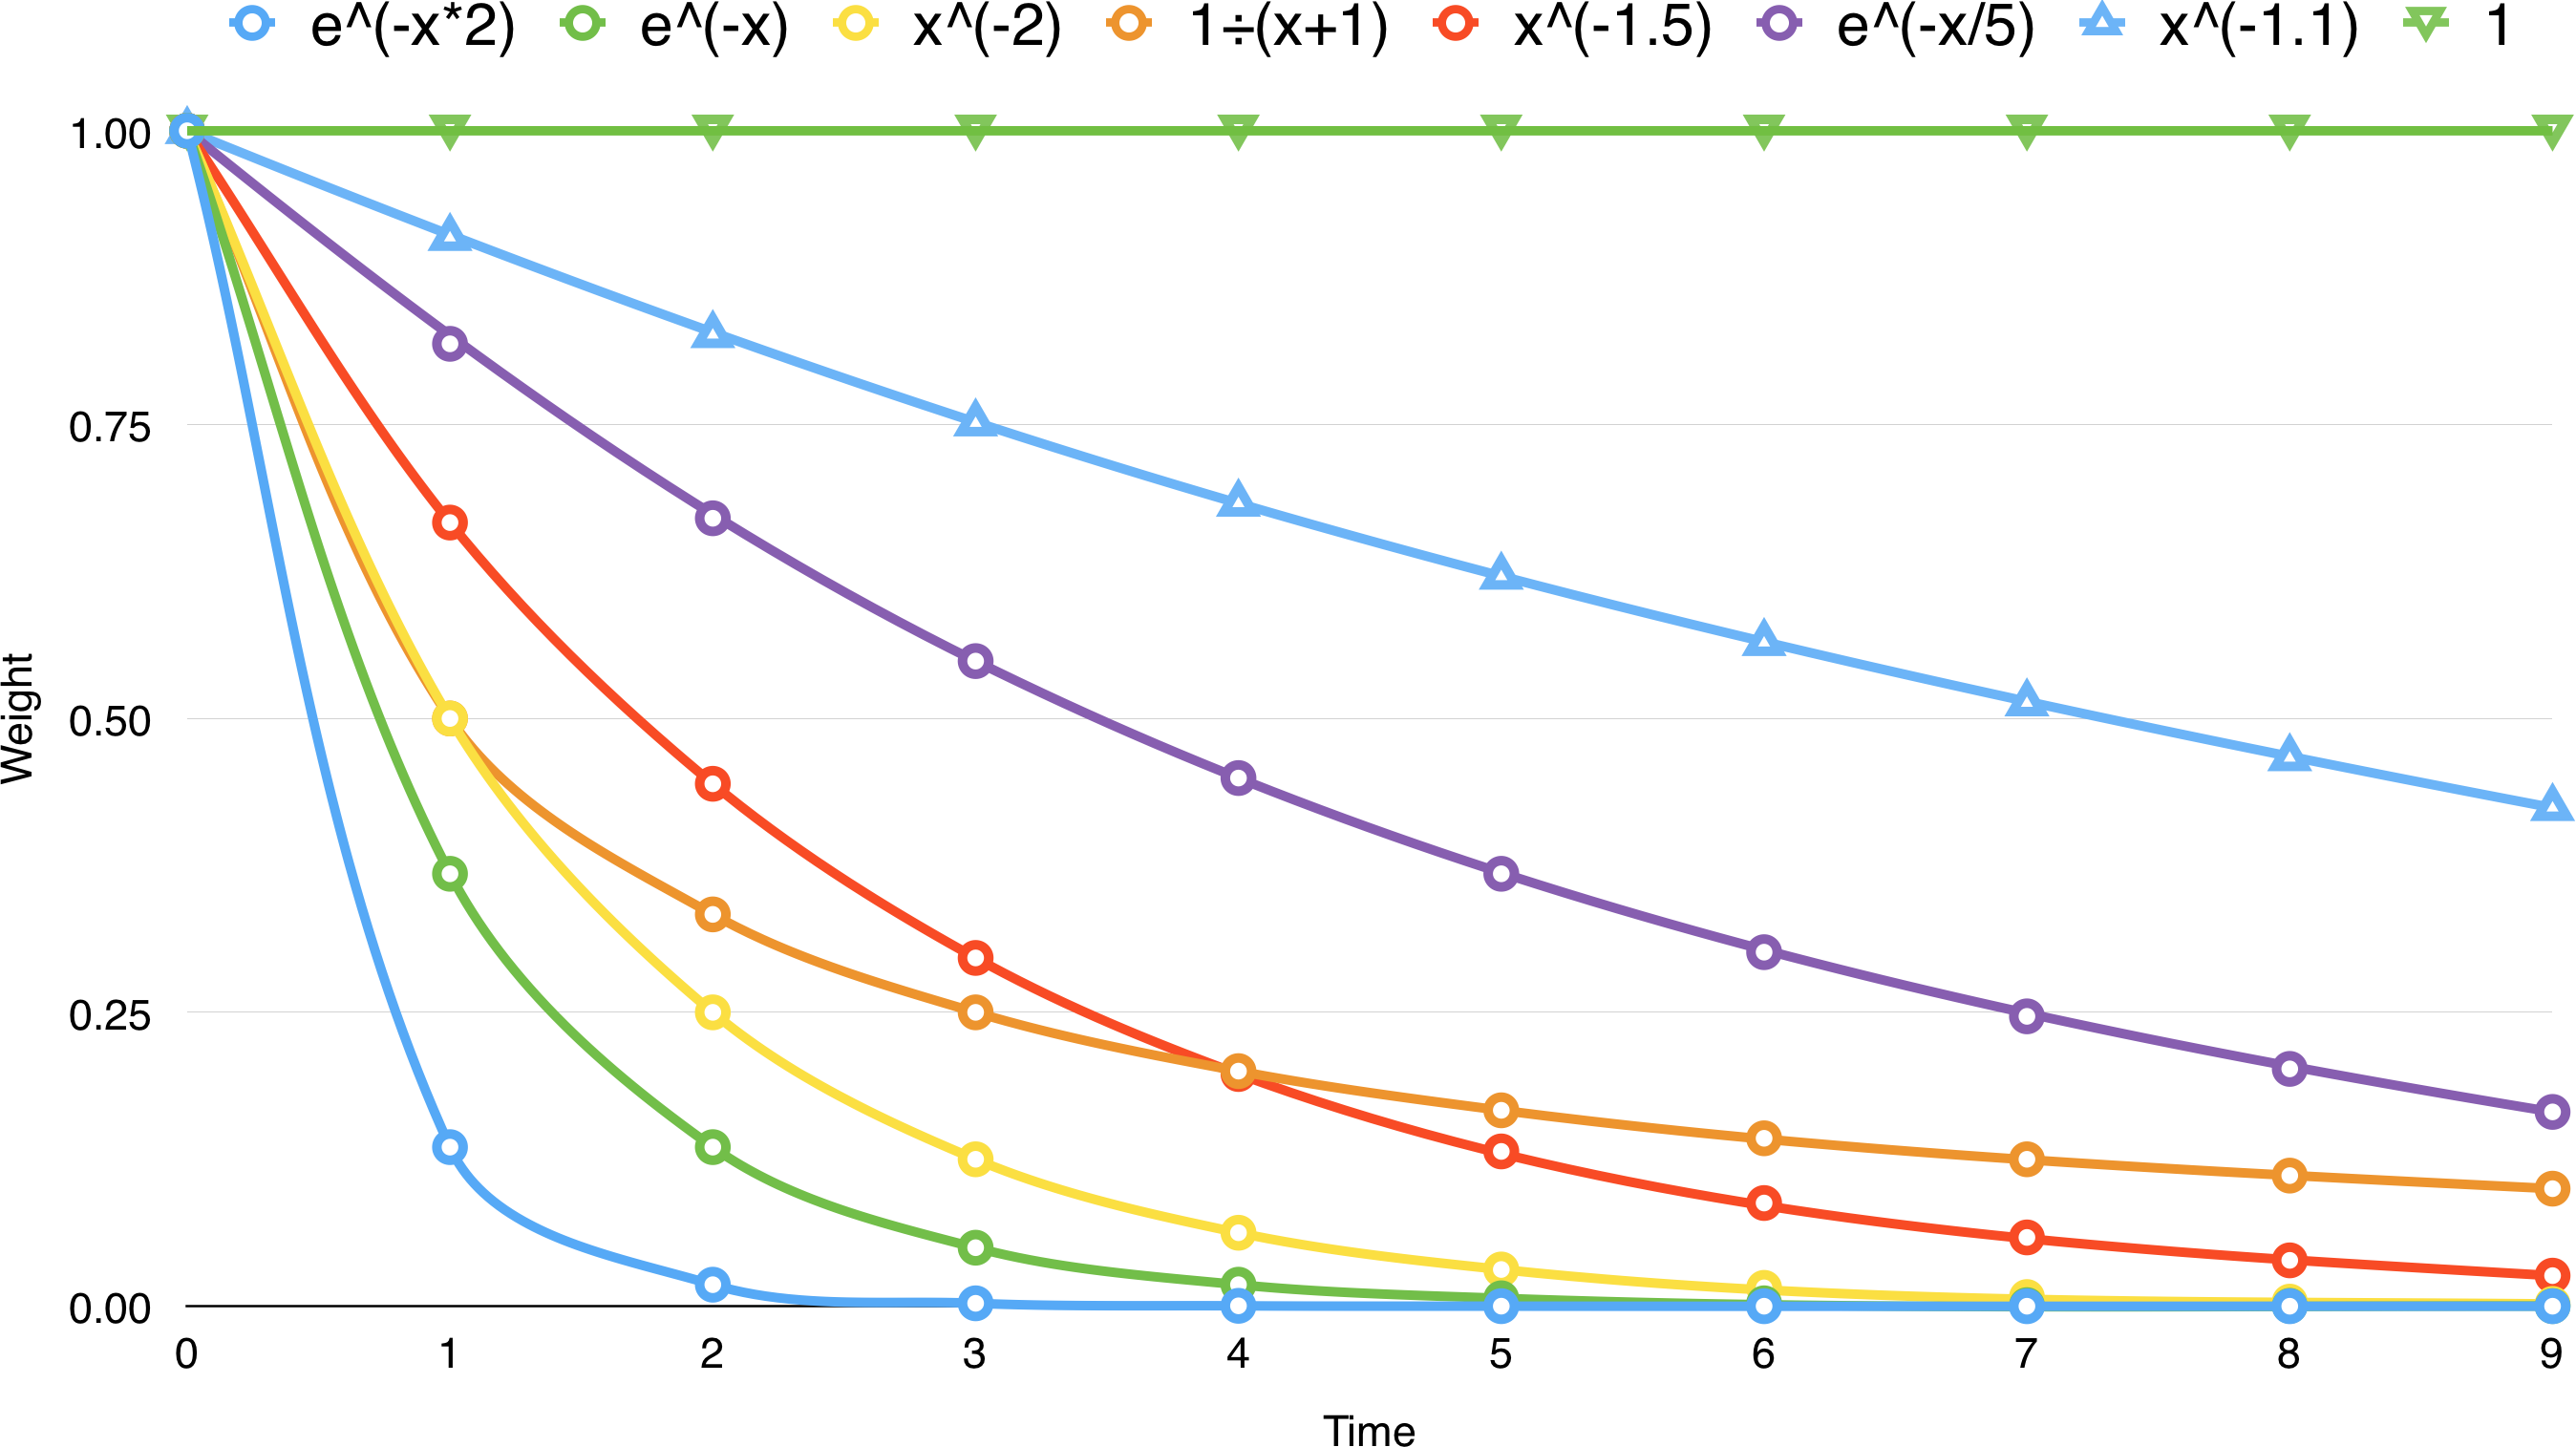
\includegraphics[width=0.9\textwidth]{design/weightedaveragesgraph}
    \caption{The eight prototype weighting functions}
    \label{fig:weightedaveragegraph}
\end{figure}

To select the best fit weighting function for each user, the system splits the complete months\footnote{Months that have passed fully} from the users transaction history into two parts. Training contains 75\% of months, starting with the oldest and the remaining 25\% (the most recent) is used for testing.
%
If less than four months are available the most recent month is used for testing and the remainder for training. In the case where between zero and two months are available the application falls back on a simple average.

Having split the data, the application loops through all the weighting functions available, calculating the weighted average of the testing data and evaluating the mean absolute error (Fig. \ref{fig:absoluteerror}) on the training data, by comparing the prediction to the actual value. The function with the least absolute error is best fit to the users overall spending pattern, and so it is selected.

In testing it was discovered that users spending money in similar categories often best suited the same weighting model. Upon further investigation it was discovered that by finding the best weighting model per category in addition to user, on average the absolute error was less. For this reason the most recent implementation of the five model system goes through a users spending in each category, selects the best model for each and uses that to make the prediction in the category. Further research could be done into different levels of modelling and the effect of this level on overfitting, this is discussed in Section \ref{section:overfittingmodels}.

\begin{figure}[h]
    \centering
    \[
        \mathrm{MAE} = \frac{1}{n}\sum_{i=1}^n \left| f_i-y_i\right| 
    \]
    \caption[Mean absolute error formula]{Mean absolute error where $f_i$ is the prediction and $y_i$ is the true value}
    \label{fig:absoluteerror}
\end{figure}

\question{Show how the one with the least error is selected?} \gavin{Yes definately}

\subsection{Confidence}
As the prediction from the Markov Chain Model is based on probabilities it is unstable. To account for this, when making a prediction, the application repeats the process of reading from the MCM up to $10,000$ times per second. The repetition of the reading is used to produce a confidence level of the final prediction once all the results are combined, which is displayed to the user. The confidence level is displayed as a plus/minus value next to the prediction and gives an indication of how sure the application is. 

Assuming the results follow a normal distribution the 95\% confidence interval is calculated by Fig. \ref{fig:confidencelevel} where $\bar{x}$ is the arithmetic mean of the predictions, $x_i$ is the value of prediction $i$ and $z$ is a value sampled from a standard normal table for the desired confidence interval.

\begin{figure}[h]
    \centering
    \[
        \bar{x} \pm z \frac{
                        \sqrt{
                            \frac{1}{n}
                            \sum\limits_{i=0}^{n}{(x_i - \bar{x})^2}
                        }
                       }{\sqrt{n}}
    \]
    \caption[Confidence Interval formula]{Confidence Interval formula}
    \label{fig:confidencelevel}
\end{figure}

\section{Security Considerations} \label{section:security}
Strong security is expected of this project. The design considers possible attack vectors and takes steps to prevent or reduce the effectiveness of those attacks.

\subsection{Account Hijacking}
To prevent the security concerns highlighted in section \ref{subsection:account-hijacking} the entire project uses HTTPS, marks cookies as HTTPS only\footnote{Using the Secure attribute}, and redirects users to the HTTPS version if they attempt to access via HTTP. This ensures user data is sent encrypted end to end and cannot be intercepted, preventing access to their authentication details or session cookie.
%
In addition cookies are marked as \inlinetext{HttpOnly}, ensuring access via non-HTTPS methods such as client side javascript is not possible. This means that even if a users browser is infected with a malicious script for example using XSS (see \ref{subsection:securityother}), the contents of the cookie cannot be read.

\begin{figure}[h]
    \centering
    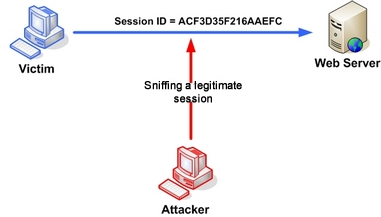
\includegraphics[width=0.6\textwidth]{design/security/sniffing}
    \caption[Obtaining a users cookie using a MitM attack or sniffing]{Obtaining a users cookie using a MitM attack or Sniffing \parencite{owasp2011sessionhihacking}}
    \label{fig:securitysniffing}
\end{figure}

\begin{figure}[h]
    \centering
    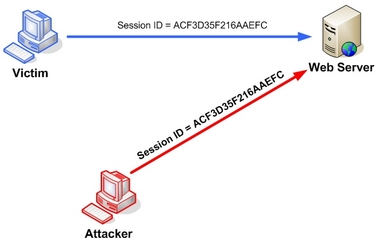
\includegraphics[width=0.6\textwidth]{design/security/hijacking}
    \caption[Performing a session hijack using another users cookie]{Performing a session hijack using another users cookie \parencite{owasp2011sessionhihacking}}
    \label{fig:securityhijacking}
\end{figure}

\subsection{Password Security}
 
The project uses Shannon's original equation, using a formula to calculate the probability of guessing each individual character. The formula takes into account that using a larger character set (such as numbers and symbols) decreases the likely hood of successfully predicting the following character and if it falls below a predefined entropy rejecting the password.
%
Enforcing an entropy threshold rather than enforcing a set of restricting `password rules', was preferred as it gives the user more flexibility hopefully avoiding the annoyance of rules and increases the search space of the passwords. A very long alphanumeric password such as `correct horse battery staple' would be just as valid as a short password containing numbers and symbols such as `6?@7a?Y5R='.

As part of a brute force attack, the attacker may use a dictionary of popular passwords to reduce the testing space before attempting an exhaustion attack.
%
In order to reduce the effectiveness of this kind of attack the project tests any user provided password against a dictionary of at least 50,000 common passwords sourced from password cracking resources \cite{burr2013electronic}.

In addition, to limit the overall effectiveness of brute force attacks, the website rate limits login attempts. If a user attempts to login more than 5 times within one minute, they must wait thirty seconds before they are able to attempt to login again.
%
Rate limiting was chosen over CAPCHA\footnote{Completely Automated Public Turing test to tell Computers and Humans Apart} found on many websites as CAPCHA's slow down users, are often illegible and visual CAPCHA's can prevent visually impaired users from accessing the website \parencite{matt2005inaccessibility, hegarty2012onlinesecurity}. Additionally CAPCHA's can now be solved automatically with a very high success rate using computer vision techniques, and these techniques are already being integrated into brute force software available online \parencite{goodfellow2013neuralnetwork, 9kweu2014captchasolver, danchev2014captcha, savinkin2012captchasolvers}. 

\subsection{Database Storage}
As detailed in section \ref{subsection:databasestorage}, security considerations of storing information in a database were considered, the project uses three techniques to help ensure the security of the users information stored in the database. \todo{Broken sentence}

\subsubsection{Passwords}
Passwords are hashed and salted and different hashing functions were investigated. Traditionally functions such as MD5, SHA1 and SHA256 are used to perform the hashing, however due to advances in modern computer equipment it is possible to generate these at an incredibly fast rate, reducing the time taken to brute force a hash.
%
Using a deliberately slow hashing function is designed avoid this problem. Blowfish written by Bruce Schneier is commonly suggested, as it is designed as a computationally expensive operation \parencite{schneier1994description} . This was evaluated with a simple test, counting the number of hashes completed in one second on the server hosting the project. Table \ref{tab:hashingspeed}, shows the results, which found that, on average, Blowfish took significantly longer to generate each hash\footnote{The code used to perform the test can be found in Appendix \ref{app:hashingtest}}.
%
For this reason the project salts all passwords and hashes them using Blowfish.

\begin{table}[h]
\begin{tabular}{llll}
         & \multicolumn{3}{l}{Hashes Per Second}                   \\
         & Average & Standard Deviation & 95\% Confidence Interval \\
MD5      & \num{2296667} & \num{12923}  & $\pm 8010$   \\
SHA1     & \num{1869725} & \num{14783}  & $\pm 9162$    \\
BLOWFISH & 17            & 0            & $\pm 0$                 \\
\end{tabular}
\caption{Comparison of hashing algorithms hash rate on a 2.7Ghz i7}
\label{tab:hashingspeed}
\end{table}

\subsubsection{Personally Identifiable Data}
Another concern is personally identifiable data being leaked. In an attempt to avoid this the application encrypts all information stored in the user table, that is needed at a later date using the AES128 encryption standard. This standard was selected for the project as was endorsed by the U.S. National Institute of Standards and Technology, when outlined by NIST in 2001 and has become the ``encryption standard for commercial transactions in the private sector'' \cite{nist2010aes, stair2009informationsystems}.

\subsubsection{Hashing of Usernames}
In addition to the encrypting of data needed at a later date, the username of each user is hashed so it is only known to the person using that account. In the rare case that any of the passwords were brute forced, the relevant username would also need to be brute forced in order to attempt a login or use the details on another website.

\subsection{Other} \label{subsection:securityother}
Other attack vectors including SQL injection\footnote{A code injection technique that uses maliciously crafted statements to modify the SQL executed} and cross-site scripting\footnote{Inserting client-side scripts to a websites HTML to customise it's logic} (XSS) were also considered.

It was decided that the project would use a prepared statements to reduce the risk of SQL injection. By sending the query followed by the parameters as literal values the database server would not interpret them as an executable portion of SQL and attacks, relying on escaping SQL such as \inlinesql{' OR 1} are prevented.

In order to mitigate the possibility of XSS the project will need to escape all content before displaying it to the user or saving to the database. It was decided that the project would use a templating language that escaped output by default, requiring the output be explicitly marked to avoid escaping.
%
By escaping all content before displaying it to the user a maliciously crafted piece of text such as \inlinehtml{<script>alert(1);</script>} would be sent to the users browser as \inlinehtml{&lt;script&gt;alert(1);&lt;/script&gt;} and not interpreted as a script.

\section{Technical Design}
It was decided that the project would be implemented as a web application. Use of a web application ensures the features of the project can be accessed from anywhere with Internet connectivity and that it is not tied to a particular piece of hardware or operating system.

\section{Language Choice}
As the project is a web application, the user interface was written in HTML \& CSS, with the interactive elements in JavaScript. PHP was used on the service side to process the user requests, render the page and access the database which was implemented using MySQL.
 
PHP was selected because the author had extensive experience in the language, it's original intended use was web development and it is well supported. It's intention of web development means it's well coupled with HTML and provides many libraries to handle it, giving the language a significant advantage over languages such as Python and Java which can be adapted for web use. A key hindrance of PHP is that is it weakly typed which lead to issues during development where objects were passed into functions expecting another object type, weakly typed languages, such as PHP, have no compile-time validation to identity this mistake. 

MySQL was selected as the database language because it's well supported by PHP and because it provides Natural Language Searching out of the box, which supports free-text queries and can calculate the relevance of a record in the database to a search term. This is used to power the suggestions feature of the website and for user entered searches.

\subsection{Design Patterns}
The project is implemented using object oriented programming (OOP). OOP is an example of a modular programing, where `Objects' have attributes and methods. In PHP objects are instances of classes, and these classes interact with each other to perform a task.

During both the design and implementation phases the General Responsibility Assignment Software Pattern (GRASP) design principles outlined by \Citeauthor{larman1997applying}  were followed when assigning responsibility to objects within the the application, these principles were designed to encapsulate well tested principles of object-oriented design and can be used to identify `good' software \parencite{larman1997applying}. \todo{Proof read this section}

\subsubsection{High Cohesion}
Cohesion is a measure of how focused the responsibility of an object is. Every object should have a highly focus purpose and only perform tasks associated with that focus. Ensuring high cohesion throughout the project results in classes are easier to understand, maintain, reuse and adapt as modification are unlikely to affect other parts of the system. High cohesion also lends itself to low coupling, another principle, which assigns responsibility to ensure low dependency between classes, that is a particular component has as little knowledge about other components as possible.

All functionality related to a particular topic has been split into separate classes and in some cases, such as the prediction system, several subclasses.

\subsubsection{Controller}
The application follows a model-view-controller pattern (MVC), which assigns responsibility of dealing with service events to a controller, encapsulates the business logic in the model and handles the user interface separately in the view. The controller is responsible for receiving the raw web requests, routing them to appropriate part of the application and then returning a rendered page to the user to be viewed in their web browser. Use of the MVC pattern is also an example of the indirection pattern, used to reduce coupling, which uses an intermediate object (the controller) as the interface between two other systems (the view and the model).

In this project, the model was split into several subsections (by functionality) to encapsulate the logic even further and these sub-models handle and manipulate the shared objects in the database. The responsibility of the objects and modules was assigned following the information expert principle, objects which hold the information necessary to complete a task, should be responsible for that task. The view is handled by a templating engine that allows the user interface to be defined in template files, rather than application logic. The output of the models is passed to the view, via the controller, which returns a complete HTML page to send to the user.

\subsubsection{Protected Variations}
The Protected Variation principle states that elements of the design that are likely to change in the future should be protected from this change by being accessed through an interface. The database access system, which is abstracted from the underlying database server, is an example of Protected Variation found in this project.

\subsection{Architecture}
The service layer of the application uses an follows a MVC request pattern, shown in Fig. \ref{fig:basic-mvc}. A HTTP request sent to the server is handled by routing, passed to the appropriate part of the controller, which interacts with the model before generating the view and returning it to the client. 

\begin{figure}[h]
    \centering
    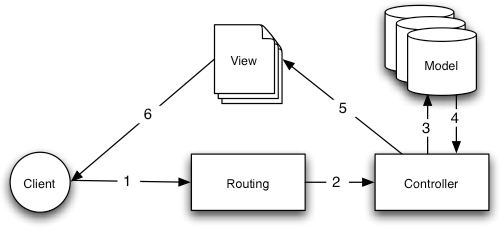
\includegraphics[width=0.6\textwidth]{design/basic-mvc}
    \caption[The MVC Request architecture of the applications service layer]{The MVC Request architecture of the application's service layer \parencite{cakephp2014mvc}}
    \label{fig:basic-mvc}
\end{figure}

The Transaction object, shown in Fig. \ref{fig:transactorcoupling}, which represents individual transactions on a users statement is the core of the applications model. It is coupled to the User, Import, Category and Transactor objects. The Import object is associated with an upload of a users statement, and contains a summary of the uploaded files contents including the date range that was found within the file. Transactions are (indirectly) associated with a Transactor, which represents a real world business that money can be sent to or from.

\begin{figure}[h]
    \centering
    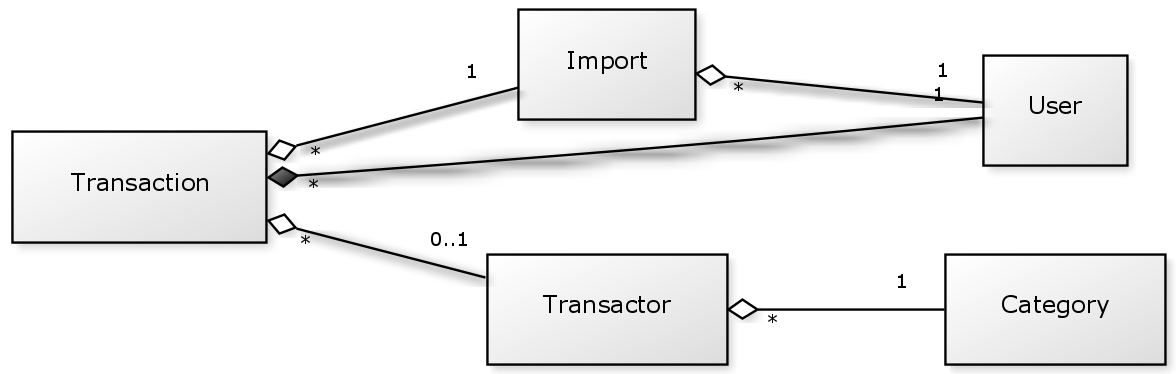
\includegraphics[width=0.8\textwidth]{design/transaction-architecture}
    \caption{Classes coupled with the Transaction object}
    \label{fig:transactorcoupling}
    
    \begin{comment}
[Transaction]<>*-0..1[Transactor]
[Transaction]++*-1[User]
[Transaction]<>*-1[Import]
[Transactor]<>*-1[Category]
[Import]<>*-1[User]
    \end{comment}
\end{figure}

A full database schema for the application is shown in \autoref{cha:databaseschema} on page \pageref{cha:databaseschema}, further examples of system architecture are shown in \autoref{subsub:wizard-implementation} and \autoref{section:prediction-implementation}.

\subsection{Project Management}
The project was developed in an iterative manner. Key pieces of functionality identified in the planning process were designed, implemented, deployed and tested first. The functionality was then reviewed by potential users, the developer and the project supervisor using lab observations and face-to-face conversations. The results of these discussions were used to decide on the next piece of functionality to implement and to adjust the plan as appropriate, restarting the process. Using an iterative method ensured that the project was build incrementally, starting with the most important features first and that a copy of the application, with the completed stable features was always available for testing and evaluation. \todo{This needs tweaking}.

The project code base was managed using the distributed version control system Git.  GitHub was selected as the host for the Git repository to keep an external backup of the code base and to access it's project management features \parencite{github2014github}.
%
Functionality and bug fix requests created during the testing and review phases were managed using the issues system (Fig.  \ref{fig:github-issues}). To start a new iteration, a milestone, containing a subset of the issues listed select by priority, was created, and this milestone was associated with a new git branch. Once the features were complete, the branch merged into the master branch, which contained a stable copy of the project at all times, and automatically deployed to the web server using post commit hooks. After completing the merge, the milestone, and all associated issues were marked complete and the process was repeated.

\begin{figure}[h]
    \centering
    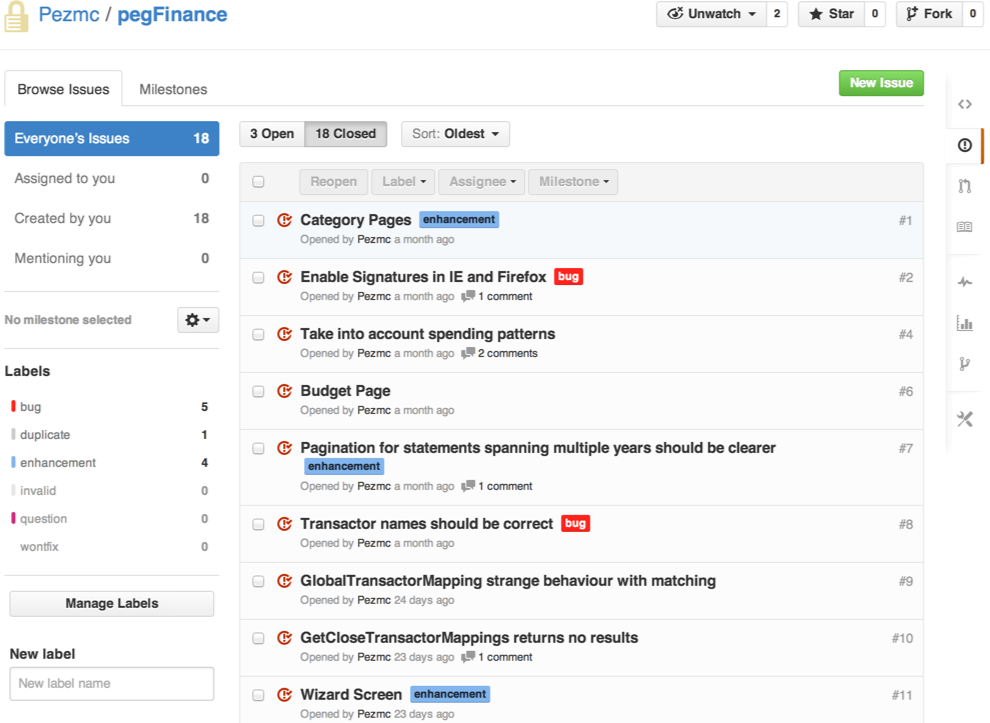
\includegraphics[width=0.8\textwidth]{design/github-issues}
    \caption{Enhancement and bug fix requests as issues on GitHub}
    \label{fig:github-issues}
\end{figure}

\chapter{Implementation}

\begin{comment}
Chapter 4: Implementation
The implementation details should be confined to the important, difficult or interesting aspects. Large chunks of code should be avoided, and diagrams and tables should be used to present details clearly.
\end{comment}

\plan{Limited to programming languages only}

This section is focused on particularly interesting parts of implementing the design outlined in \autoref{cha:design} or external libraries.

\section{Languages}
As it was decided the project would be a web application\todo{Should probably mention this in design} the user interface was written in HTML \& CSS, with the interactive elements such as the graphs in JavaScript. PHP was used on the service side to process the user requests, render the page and access the database which was implemented using MySQL.
 
PHP was selected because the author had extensive experience in the language, it's original intended use was web development and it is well supported. It's intention of web development means it's well coupled with HTML and provides many libraries to handle it, giving the language a significant advantage over languages such as Python and Java which can be adapted for web use. A key disadvantage of PHP is that is it weakly typed which lead to some issues during development where objects were passed into functions expecting another type, weakly typed language have no compile time validation for this mistake. This disadvantage was considered and it was decided the advantages outweighed the disadvantages.

MySQL was selected as the database language because it's well supported by PHP and because it provides Natural Language Searching out of the box, which supports free-text queries and can calculate the relevance of a record in the database to a search term. This is used to power the suggestions section of the website and for user entered searches.

\section[Key Libraries]{Key External Libraries}
A full list of external libraries and frameworks used by the project can be found in \autoref{app:externallibraries}.

\subsection{Server Side}
\subsubsection{Framework}
The project uses a PHP Framework, written by the report author, to handle functionality that is common across different web applications, including request routing, template generation and caching.

Using the framework has several key advantages over writing the whole system from scratch:

\begin{itemize}
\item[Model View Controller] MVC is enforced ensuring ensures models (data structures), views (page content) and controllers are separate, improving cohesion and decreasing coupling
\item[Code Structure] Code is structured in a standardised manner, split by functionality and is not executable over the web
\item[Rapid Code Development] Functionality such as routing, security and caching, that is common between web applications is already implemented
\item[Vendor Libraries] External libraries supported by the framework can be used without additional code, such as Twig, the template engine
\end{itemize}

\subsubsection{Twig}
Twig is a PHP template engine that takes collections of PHP objects and following a provided .html template generated the HTML output that is ultimately sent to the browser. Although PHP itself is by design a template engine, using a dedicated templating engine allows separation of concerns and addresses the shortcomings of PHP as a template language.

Twig includes idioms for common needs including a \inlinetext{for/else} structure which loops through a list or, if that list is empty, evaluates the else clause and template inheritance; is unit tested; caches all generated templates leading to significant speed increases for the end user and provides shorthand filters such as \inlinephp{[1, 2, 3, 4]|first} but most importantly, escaping is enabled by default. In twig all data output as part of a template is converted to the equivalent HTML entity so it cannot be parsed as a script or HTML.
% 
A comparison of Twig and PHP for a simple page containing a for loop and output escaping is shown in Fig \ref{fig:comparephptwig}.

\begin{figure}
\centering

\begin{subfigure}[a]{\textwidth}
\centering
\begin{lstlisting}[style=phpcolor]
<?php if($items): ?>
  <?php foreach($items as $item): ?>
    * <?php echo htmlspecialchars(strtoupper($item->name), ENT_QUOTES, 'UTF-8') ?>
  <?php endforeach; ?>
<?php else: ?>
    No item has been found.
<?php endif; ?>
\end{lstlisting}
\caption{PHP as a Templating Engine}
\end{subfigure}

\begin{subfigure}[b]{\textwidth}
\centering
\begin{lstlisting}[style=phpcolor,language=twig]

  * {{ item.name }}

  No item has been found.

\end{lstlisting}
\caption{TWIG as a Templating Engine}
\end{subfigure}

\caption{Comparison of TWIG and PHP for a simple template}
\label{fig:comparephptwig}
\end{figure}

Twig was selected over alternative engines as it is both well documented and supported, supports extensions out of the box which can be used to add additional functionality and as shown in Table \ref{table:twigbenchmarked} is by far the fastest when compared to alternatives \parencite{potencier2009templating}.

\begin{table}[h]
\begin{tabular}{llll}
\textbf{Library} & \textbf{Time (sec)} & \textbf{Memory (Kb)} & \textbf{Templates rendered per second} \\
Twig             & 3                   & 1,190                & 3,333                                  \\
PHPTAL           & 3.8                 & 2,100                & 2,632                                  \\
Dwoo             & 6.9                 & 1,870                & 1,449                                  \\
Smarty 2         & 12.9                & 2,350                & 775                                    \\
Smarty 3         & 14.9                & 3,230                & 671                                    \\
Calypso          & 34.3                & 620                  & 292                                    \\
eZ Templates     & 53                  & 5,850                & 189                                   
\end{tabular}
\caption[PHP Templating engine benchmarks]{PHP Templating engines compiling and rendering a simple page 10,000 times \parencite{potencier2009templating}}
\label{table:twigbenchmarked}
\end{table}

\subsubsection{Propel}
Propel is an object relational mapping (ORM) library for PHP, which allows the storing and loading objects to and from a relational database.
%
Propel takes, a database schema defined in XML and generates PHP objects that representing the schema which can be saved to, and loaded from, the database \parencite{propel2014orm}.

Use of an ORM has four main advantages, it abstracts the database layer providing a common interface protecting against change, it allows for business logic to be  encapsulated in the generated objects and not the database, it helps address the cross cutting concerns of database access and wraps common database design patterns in easy to access functions. In addition to these common ORM features, Propel wraps object inheritance in an API, for example to get all the transactions that a user has made \inlinephp{$user->getTransactions()} is called which returns an array of Transaction objects.

\subsection{Client Side}
\subsubsection{Bootstrap}
Bootstrap is a CSS framework for creating user interfaces. It provides a grid layout system, pre-designed reusable components such as buttons; implements common CSS design patterns and supports responsive web design, as well as gracefully degrading when using older browsers or mobile devices \parencite{bootstrap2014bootstrap}.

An extended version of bootstrap is used for the front end of the project, though the colour scheme and layout has been heavily modified to ensure the application doesn't look like a `Bootstrap website' which is a common complaint of web designers and to ensure a common brand \parencite{kizler2013bootstrap, carrico2013bootstrap}.

\subsubsection{jQuery}
jQuery is a JavaScript development framework that abstracts differences in browser behaviour and provides shorthands to common JavaScript tasks such as AJAX requests, element selection, and HTML traversal and manipulation.
%
It's used throughout the website for javascript user interface effects and powers the core of the  suggestion wizard, which is detailed further in \autoref{subsection:suggestionwizard}.
%
It was chosen for the project over other JavaScript frameworks as it is; extendable, open-source, , provides method chaining and is supported by large respected companies on the web including Google and Microsoft \parencite{jquery2014jquery}.

\section[Statements]{Statement Management}

\subsection{Upload}
OFX is an XML like format called SGML. PHP has inbuilt libraries for parsing XML called SimpleXML simplexml\_load\_string loads an XML file from a string. To parse the OFX, PHP attempts to parse it as an XML file and captures any exceptions. If exeptions are found it attempts to convert the SGML XML so it can be pased by PHP as per \todo{This needs completing}

%http://stackoverflow.com/questions/15735330/how-to-parse-a-ofx-version-1-0-2-file-in-php and http://www.hanselman.com/blog/PostprocessingAutoClosedSGMLTagsWithTheSGMLReader.aspx

\todo{Comparison of SGML and XML}

For each line of the SGML it trims whitespace including (x,y,z), converts the charset ot UTF-8 so it's valid in PHP and if no closing tag is found, appends a closing tag

\begin{figure}
\lstset{style=phpcolor}
\begin{lstlisting}
foreach(preg_split("/((\r?\n)|(\r\n?))/", $this->OFXContent) as $line){
        		
        	// Trim whitespace
        	$line = trim($line);
        	if ($line === '') continue;
        
        	// Convert charset to UTF-8
        	$line = iconv($charset, 'UTF-8', $line);
        	if (substr($line, -1, 1) !== '>') {
        		list($tag) = explode('>', $line, 2);
        		$line .= '</' . substr($tag, 1) . '>';
        	}
        	$buffer .= $line ."\n";
}
\end{lstlisting}
\caption{Converting SGML to XML}
\end{figure}

Having parsed the SGML into objects it can just be navigated following the specification and converted to arrays of information for each transaction, refered to as movements. These movements look like XYZ; and can then be convered into the Transaction objects most of the fields are handled automatically but dates need to be handled specifically.

QIF is handled in a different manor as there are no native libraries to parse it's format. As per the Fig. \ref{fig:qifofxformat} shown in section \ref{subsection:upload} shown in  the format is a list of individual movements, with each terminated a \^. Each field associated with an individual movement is identified with a letter, explaining the contents of that line.
% 
The field types that the project was interested in and parses are shown in Table \ref{table:qiffields}.

\begin{table}[h]
\centering
\begin{tabular}{ll}
D                  & Date           \\
T                  & Amount         \\
C                  & Cleared status \\
P                  & Payee          \\
M                  & Memo           \\
\textasciicircum   & End of entry  
\end{tabular}
\caption{QIF fields parsed by the project}
\label{table:qiffields}
\end{table}

In a similar manner to parsing the OFX files, the application loops though all the lines found in the file, switching on the identifier and sorting the information into an array representing that movement. 

\begin{figure}
\lstset{style=phpcolor}
\begin{lstlisting}
$id = substr($line, 0, 1);
$content = trim(substr($line, 1));

switch ($id) {
	case '^': // End of entry
		$this->movements[] = $newMovement;
		$newMovement = array();
		break;
		
	case 'T': 	// Amount
		$newMovement["value"] = floatval(preg_replace("/[^0-9.-]/", "", $content));
		break;
		
	case 'D': 	// Date
		$newMovement["date"] = $content;
		break;
		
	// etc ...
\end{lstlisting}
\caption{Parsing QIF transactions using the line identifier}
\end{figure}

As outlined in section \ref{subsection:upload} the conversion from the array to a Transaction object is slightly more involved due to unknown date format. To implement this in PHP, before beginning the conversion, all movements are tested against two regular expressions (regex), representing the possible formats of the dates, which are visualised as graphs in Fig. \ref{fig:regex-dmy} and \ref{fig:regex-mdy}. 
%
Having considered all the movements found in the file, the application has either decided on one of the date formats or prompts the user to decide the appropriate format, as seen in Fig. \ref{fig:dateformat-prompt}.

\begin{figure}
\lstset{style=phpcolor}
\begin{lstlisting}
$dmy = true;
$mdy = true;
foreach($this->getMovements() as $movement)
	if(!preg_match('#(0[1-9]|[12][0-9]|3[01])[-/](0[1-9]|1[012])[-/](19|20|21)?\d\d#', $date))
		$dmy = false;
	
	if(!preg_match('#(0[1-9]|1[012])[-/](0[1-9]|[12][0-9]|3[01])[-/](19|20|21)?\d\d#', $date))
		$mdy = false;
\end{lstlisting}
\caption{Identifying the date format using regular expressions}
\end{figure}

\begin{figure}[h]
    \centering
    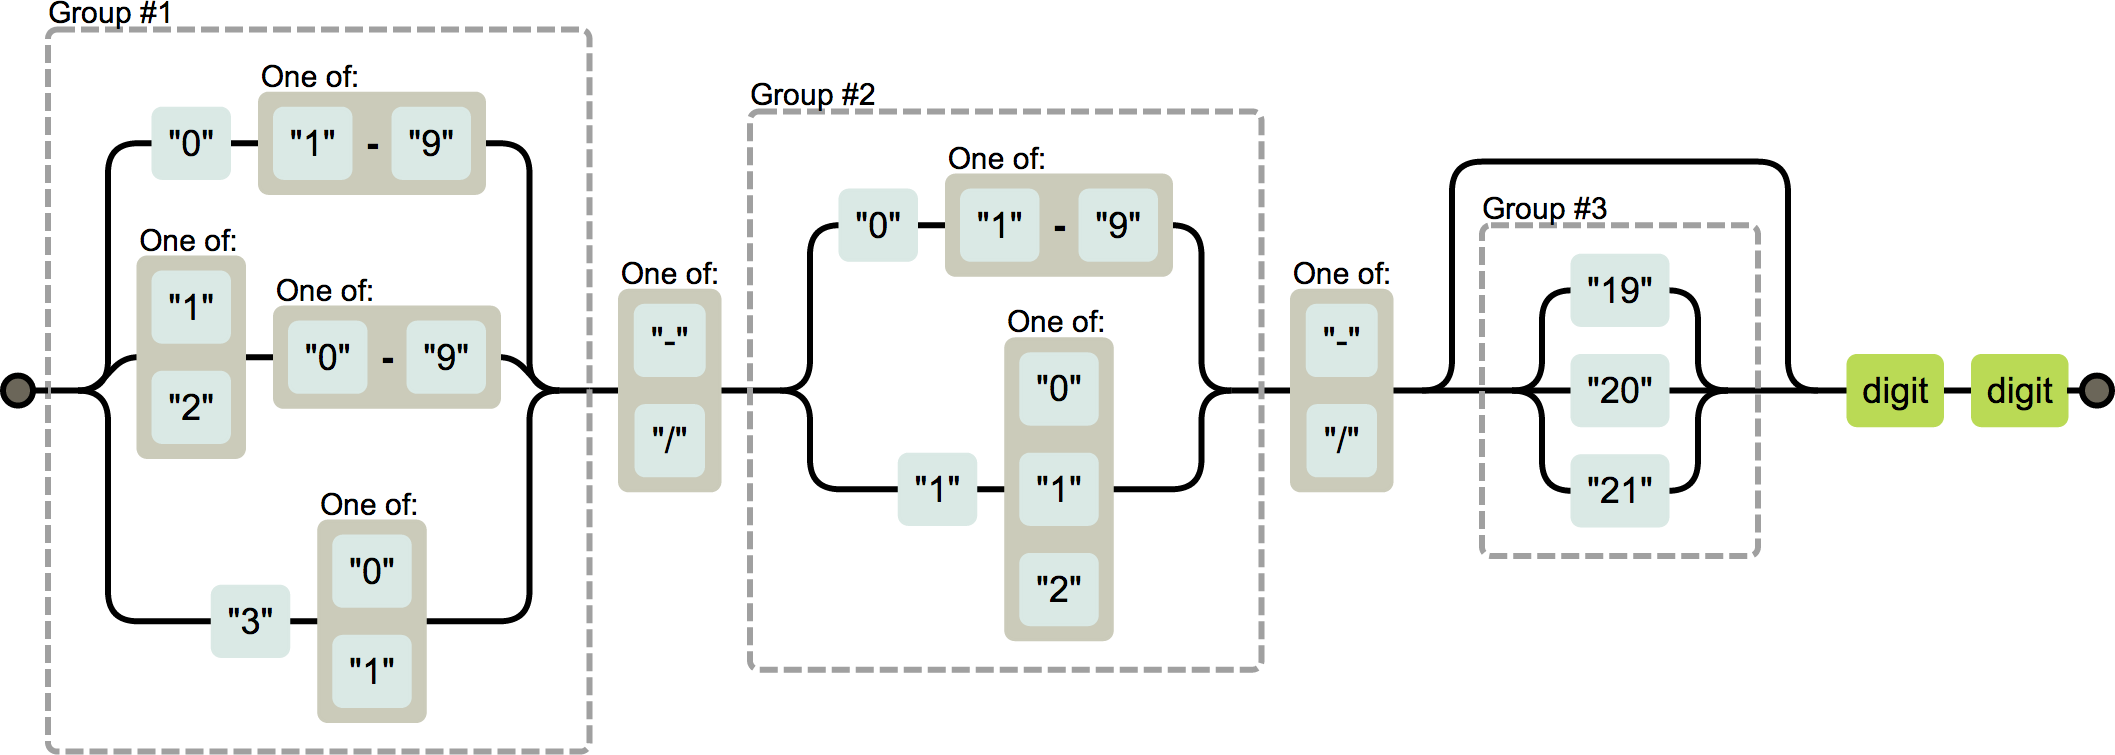
\includegraphics[width=\textwidth]{implementation/regex-dmy}
    \caption[Regular expression used to match d-m-Y]{Railroad diagram of the regex used to match format d-m-Y}
    \label{fig:regex-dmy}
\end{figure}

\begin{figure}[h]
    \centering
    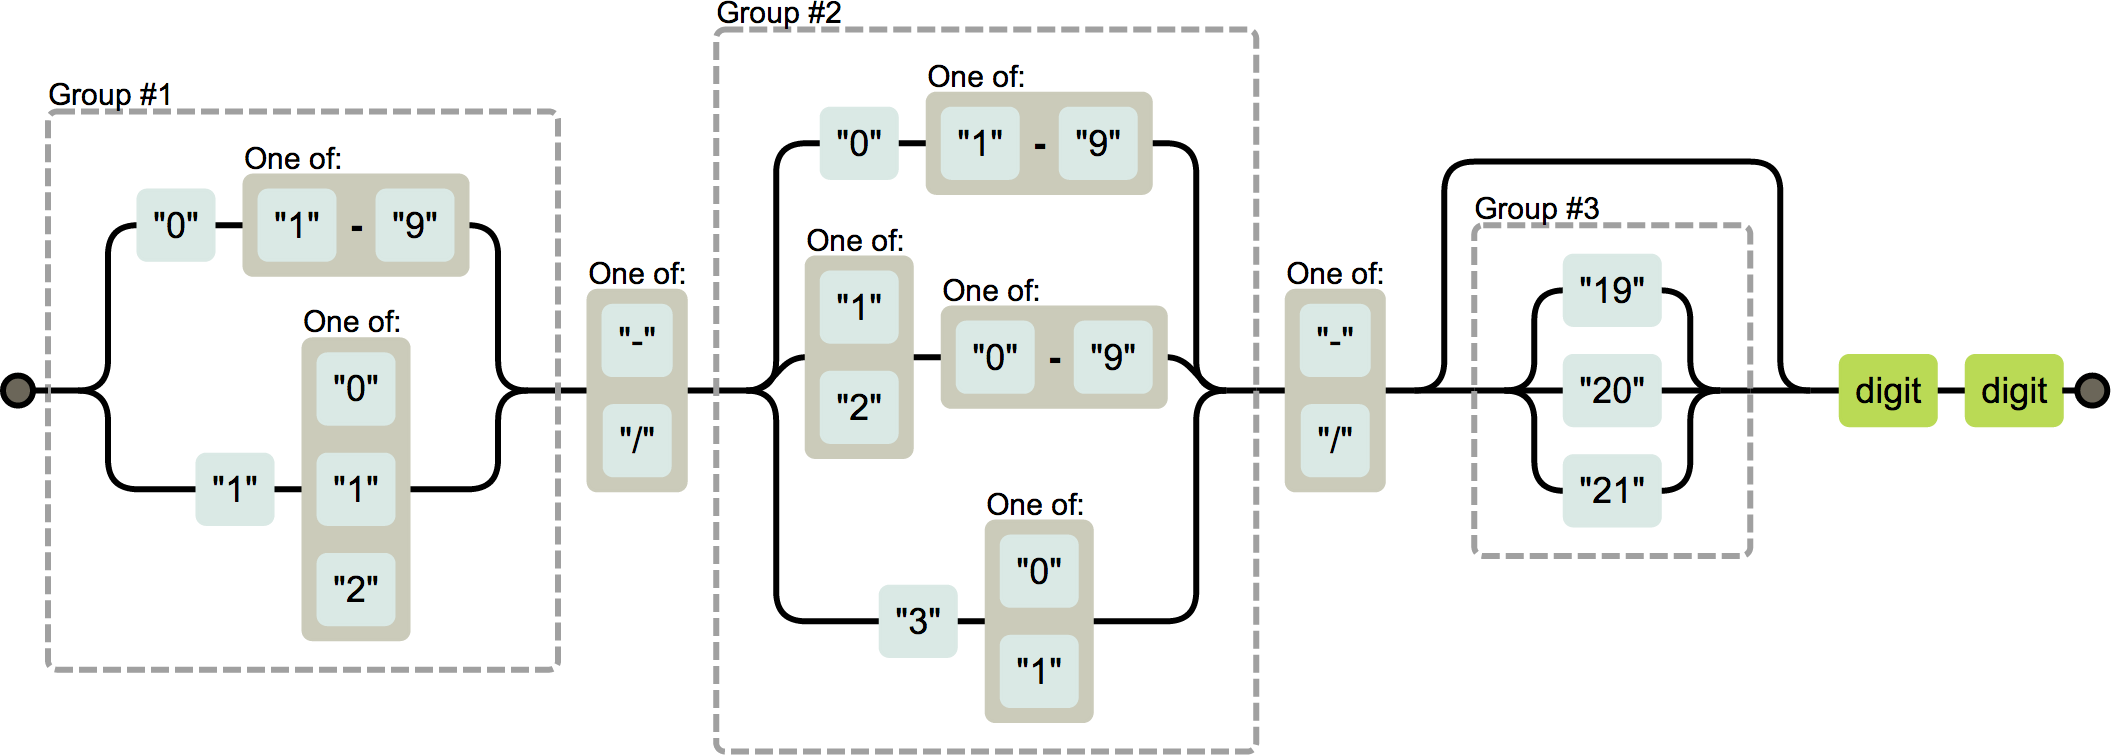
\includegraphics[width=0.75\textwidth]{implementation/regex-mdy}
    \caption[Regular expression used to match m-d-Y]{Railroad diagram of the regex used to match format m-d-Y}
    \label{fig:regex-mdy}
\end{figure}

\begin{figure}[h]
    \centering
    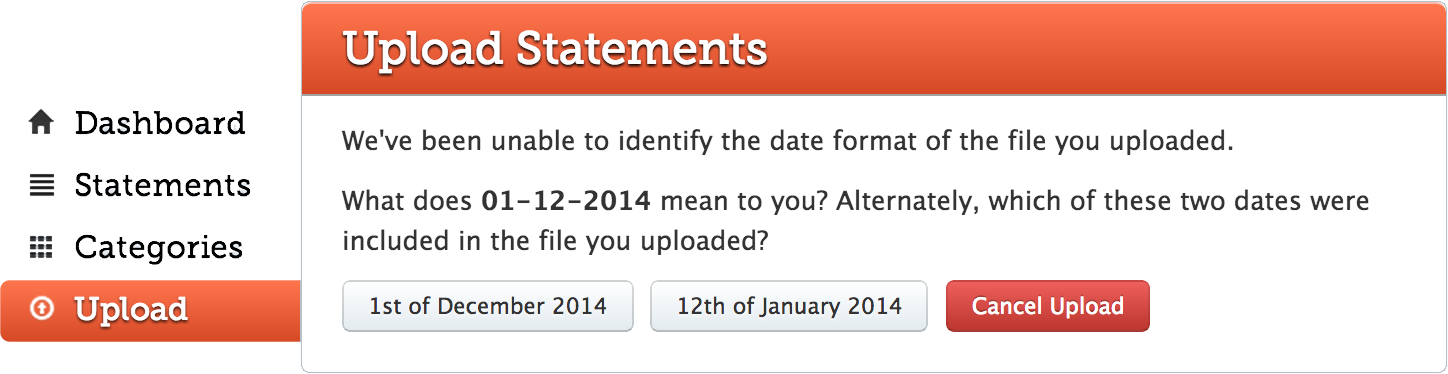
\includegraphics[width=0.70\textwidth]{implementation/dateformat-prompt}
    \caption[UI Prompt asking for date format]{UI Prompt when the application is unable to decide an upload's date format}
    \label{fig:dateformat-prompt}
\end{figure}

\subsection{Named Entity Resolution}
The implemented the mapping architecture outlined in the design, the majority of the named entity resolution is done in the \lstinline{setTransactor} method of the Transaction object, which is called when setting the name of transactor for a each transaction found in the uploaded file.   
% 
The method performs three key actions, tidying the string, removing common notation added by banking institutions and checking the database for known user and global transactors, otherwise creating a new one.
% 
To avoid unnecessary duplication in the mappings table the \gls{transactor} names are normalised before checking for an existing name, this normalisation was added to combat the various different ways which banks store the transactor names which were discovered during testing. The modifications included: padding with spaces, replacing spaces with underscores/tabs, or including non alphanumeric letters; some examples are shown in Table \ref{table:cleaningstrings}.
%
Having normalised the input, the next step was to remove any numeric identifiers which had been added and move that detail to another field. Examples of such identifiers included store id's for shops with multiple outlets and account numbers for transfers between accounts, if this detail wasn't removed a separate mapping would be created for transactions referencing the same entity, leading to unnecessary duplication. The identifiers were removed using a regex, expressed in Fig. \ref{fig:regex-transactor} which only captures numbers found at the end of the string requiring at least two digits, these additional constraints were added to preserve \glspl{transactor} with numbers in their name, such as \inlinetext$H3G$ and \inlinetext$SUPERMERCADO 3$.
%
The final step checks for existing \glslink{globaltransactor}{GlobalMapping} or \glslink{usertransactor}{UserMapping} objects in the database and if found associates that mapping with this transaction. If neither mapping's are found a new \glslink{usertransactor}{UserMapping} object is created, persisted and associated with the transaction. Differing from the original plan, fuzzy matching\footnote{ Finding strings that approximately rather than exactly match} of the transactor name when searching for existing transactors is not performed as this functionality was moved to the suggestion wizard.
%
The full code for the `setTransactor` method is shown in Fig. \ref{fig:settransactor}.

\lstset{language=textwithspaces,style=showspaces}
\begin{table}[h]
\centering
\begin{tabular}{ll}
Raw Transactor Name & Occurrences \\
\inlinetext$TESCO STORES 5128$   & 87         \\
\inlinetext$TESCO STORES 2977$   & 68         \\
\inlinetext$TESCO_STORES$        & 14         \\
\inlinetext$SACAT MARKS    AND$  & 33         \\
\inlinetext$SACAT MARKS  AND$    & 16         \\
\inlinetext$WILKINSON $          & 22         \\
\inlinetext$WILKINSON$           & 8          \\        
\inlinetext$TO A/C 00000000$\footnote{Account number removed} & 2  
\end{tabular}
\caption{Examples of the raw transactor names found on uploaded statements}
\label{table:cleaningstrings}
\end{table}

\begin{figure}[h]
    \centering
    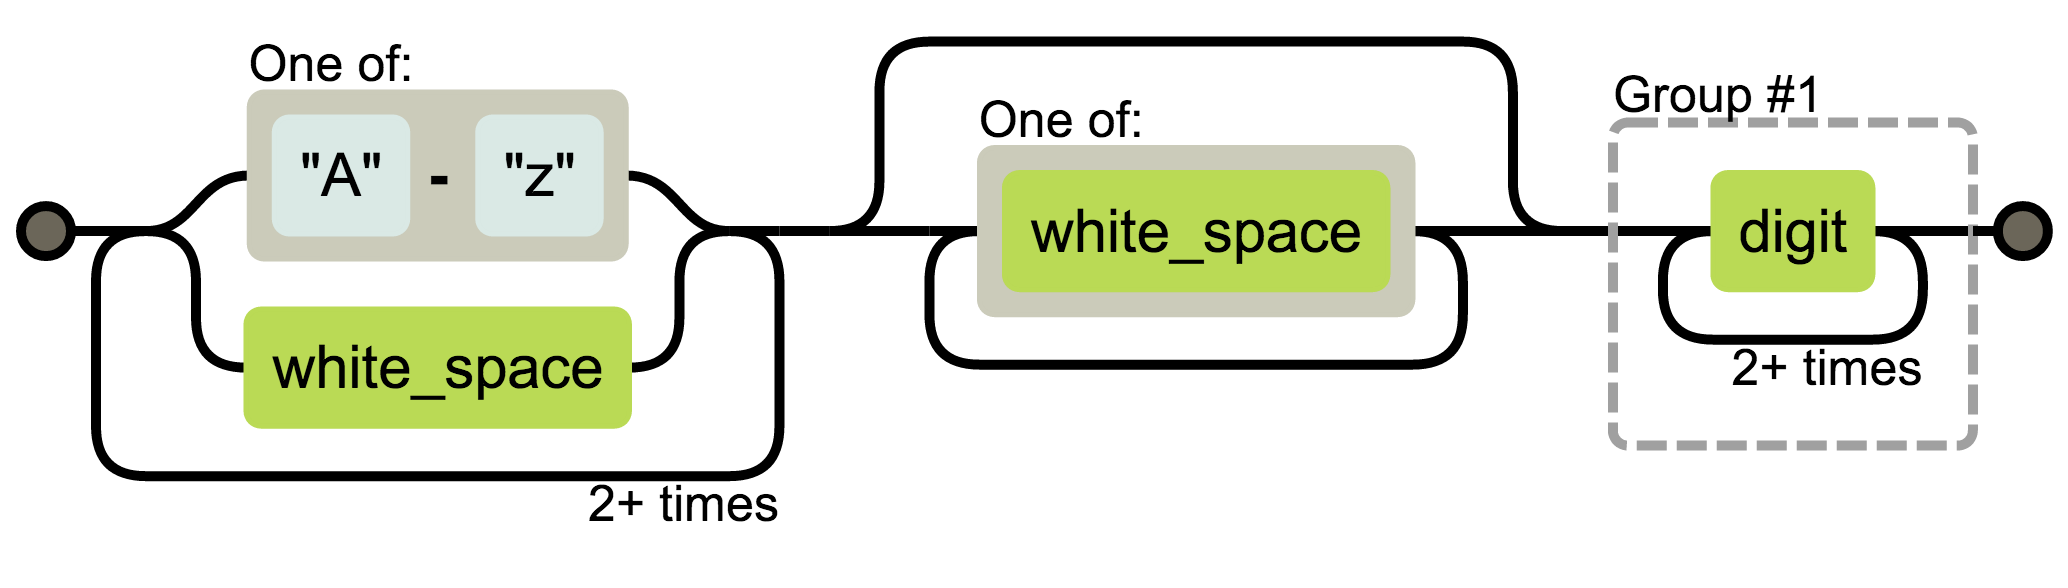
\includegraphics[width=\textwidth]{implementation/regex-transactor}
    \caption[Regular expression used to match the transactor name]{Railroad diagram of the regex used to tidy the transactor name}
    \label{fig:regex-transactor}
\end{figure}

\subsection{Suggestion Wizard} \label{subsection:suggestionwizard}
The suggestion wizard (Fig \ref{fig:suggestion-wizard}) was added to the project in response to observations during lab usability testing. Originally the suggestions were only found on each unmapped transactors page (Fig. \ref{fig:view-reference-suggestions}) to speed up the process of mapping a reference to an existing transactor.  Users appeared to spend a lot of time manually categorising each individual transactor by searching their statement for an unknown transactor, opening that transactors details and then filling in the appropriate forms or clicking on a suggestion, following an activity diagram similar to Fig. \ref{fig:transactor-mapping-activity}.

\begin{figure}[h]
    \centering
    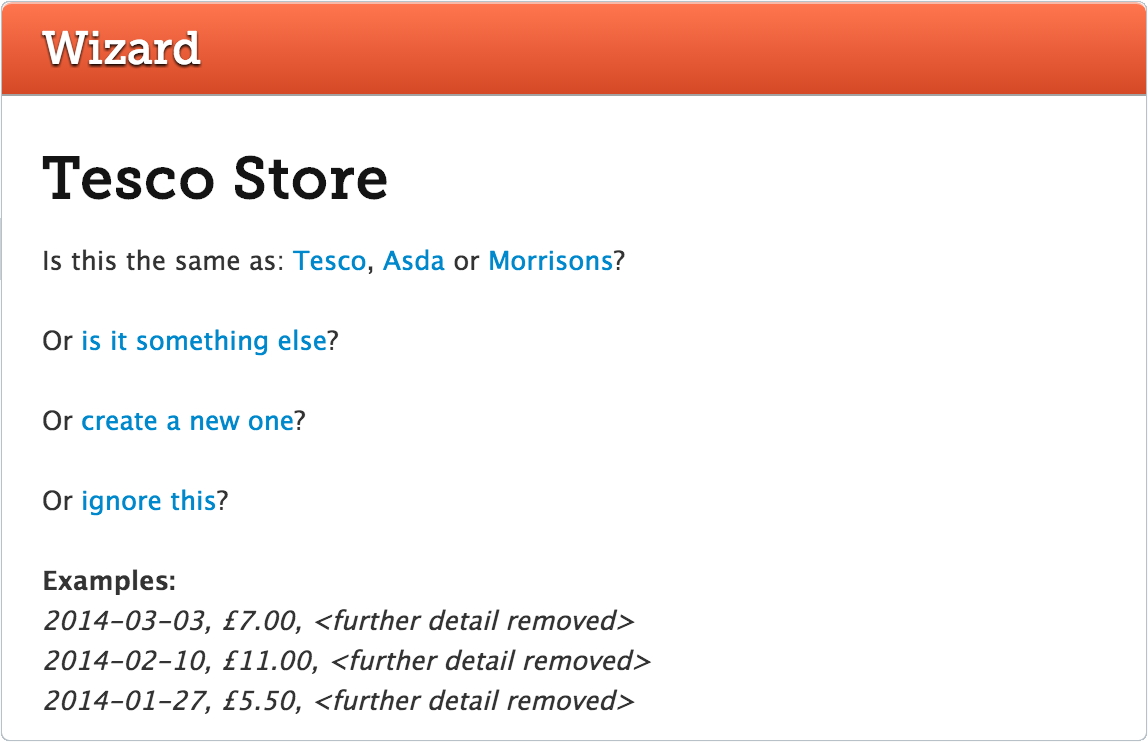
\includegraphics[width=0.75\textwidth]{implementation/suggestion-wizard}
    \caption[Suggestion wizard UI]{Suggestion wizard UI\protect\footnotemark}
    \label{fig:suggestion-wizard}
\end{figure}
\footnotetext{Potentially personally identifiable information removed}

\begin{figure}[h]
    \centering
    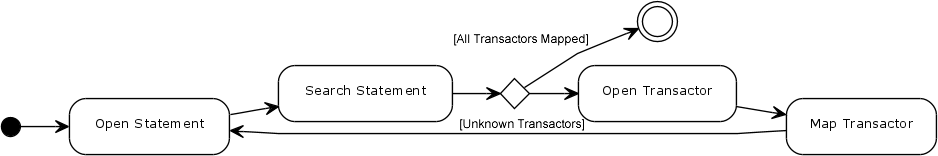
\includegraphics[width=\textwidth]{implementation/transactor-mapping-activity}
    \caption{Activity diagram for mapping individual transactors}
    \label{fig:transactor-mapping-activity}
    
    \begin{comment}
(start)->(Open Statement)->(Search Statement)-><a>->(end)
<a>->(Open Transactor)->(Map Transactor)->(Open Statement)
    \end{comment}
\end{figure}

\begin{figure}[h]
    \centering
    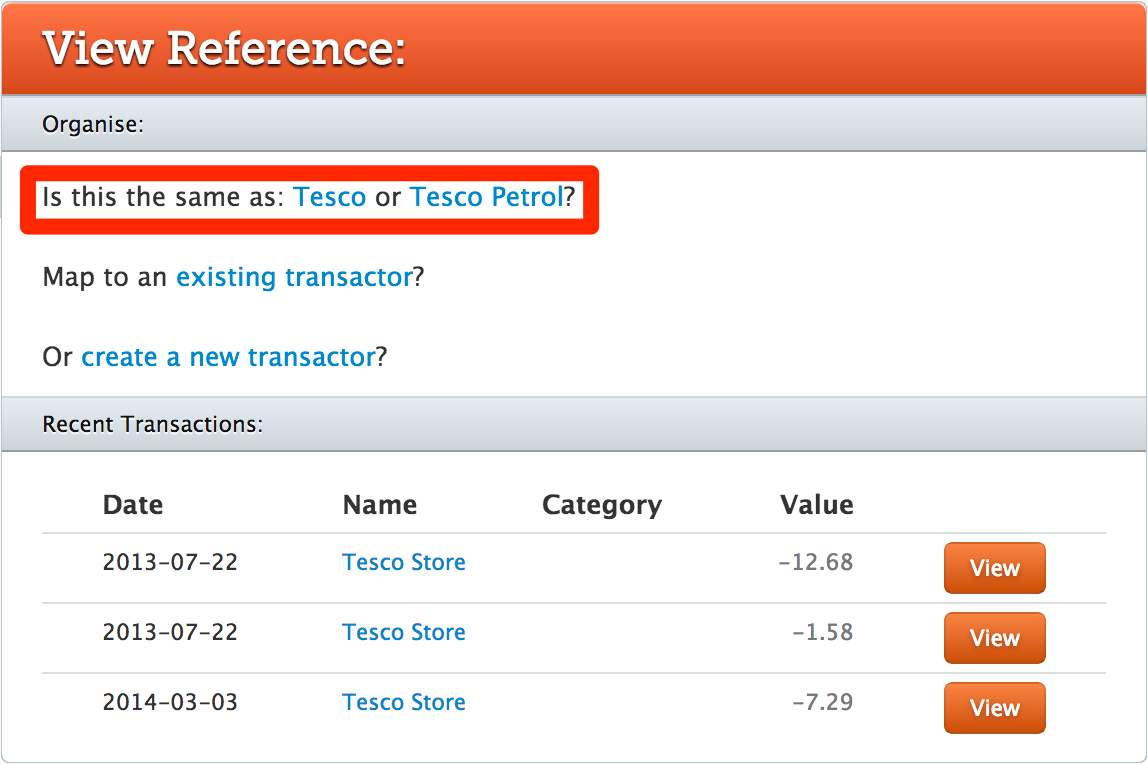
\includegraphics[width=0.75\textwidth]{implementation/view-reference-suggestions}
    \caption{Suggestions shown on the Transactor (reference) page}
    \label{fig:view-reference-suggestions}
\end{figure}

The wizard was designed to streamline and speed up this process as well as making it easier for the user to follow. Each unmapped transactor is displayed in turn, starting with the one with the most transactions (encouraging the user to map the ones they shop at more often first). On each step, the user can; follow the suggestions, manually map the reference to an existing transactor, create a new transactor or ignore the reference for now. A step-by-step view of this process is shown in section \ref{subsection:suggestion-wizard-walkthrough}.

During the process feedback is displayed to the user using notifications that appear over the wizard and are coloured according to validation style convention, with red warning of an error and green confirming success (Fig. \ref{fig:suggestion-notification}). 
%
The notifications themselves were implemented using the PNofity javascript library for jQuery which provides an API for managing alerts send to the user. PNotify was chosen as it had native support for bootstrap styles, which were already being used for the projects UI, and it was open source licensed under the GPL\footnote{GNU General Public License \parencite{gnu2007license}} \parencite{huber2014potify}.

\begin{figure}[h]
    \centering
    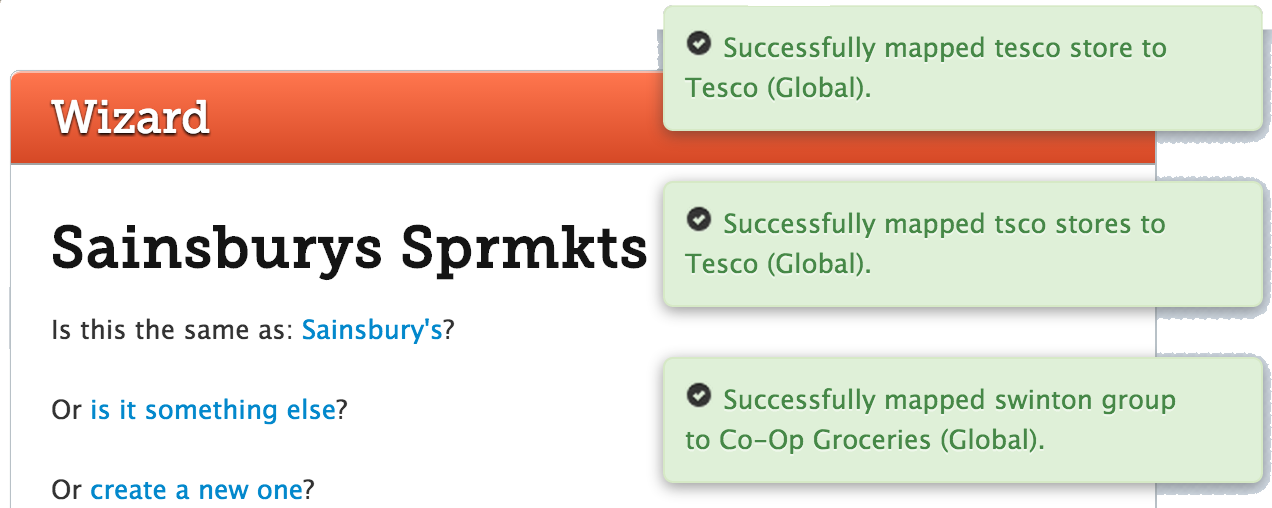
\includegraphics[width=0.75\textwidth]{implementation/suggestion-notification}
    \caption{Notifications shown during the suggestion wizard}
    \label{fig:suggestion-notification}
\end{figure}

By following the wizard users are able to quickly map the majority of their transactions in an easy to follow way, as can be shown by the activity diagram in Fig. \ref{fig:suggestion-wizard-activity}.

\begin{figure}[h]
    \centering
    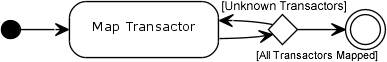
\includegraphics[width=0.6\textwidth]{implementation/suggestion-wizard-activity}
    \caption{Mapping transactors using the suggestion wizard}
    \label{fig:suggestion-wizard-activity}
    
    \begin{comment}
(start)->(Map Transactor)-><a>->(end)
<a>->(Map Transactor)
    \end{comment}
\end{figure}

The wizard is powered by Ajax\footnote{Asynchronous JavaScript and XML}, which sends requests to a backend RESTful API which proves access to the unmapped transactors found for the user. The requests and responses are sent as JSON\footnote{JavaScript Object Notation} which is supported natively by both PHP and JavaScript. A GET request to \lstinline{/ajax/transactor/suggestions} returns a collection of unmapped transactors including associated examples which are then added to the UI using JavaScript.
%
Mapping (including following a suggestion) and creating a new transactor are both handled by POST requests to the same API. Mapping sends a request to \lstinline{/ajax/transactor/map} containing the ID of the user mapping and global mapping  and creation sends a request to \lstinline{/ajax/transactor/create} including the user mapping ID to associate with the new transactor. 
%
Examples of the JSON communication are shown in Fig. \ref{fig:json-examples}.

On the backend, all JSON serialisation is handled by implementing the \inlinephp{JsonSerializable} interface on all objects that need to be JSON encoded. This allows the native function \inlinephp{json_encode(\$object)} to correctly encode the object into JSON using the data returned by the abstract method `jsonSerialize` defined in the interface. The final inheritance diagram for the mapping, transactor and transaction objects is shown in Fig. \ref{fig:mapping-inheritance-diagram}.

\begin{figure}[h]
    \centering
    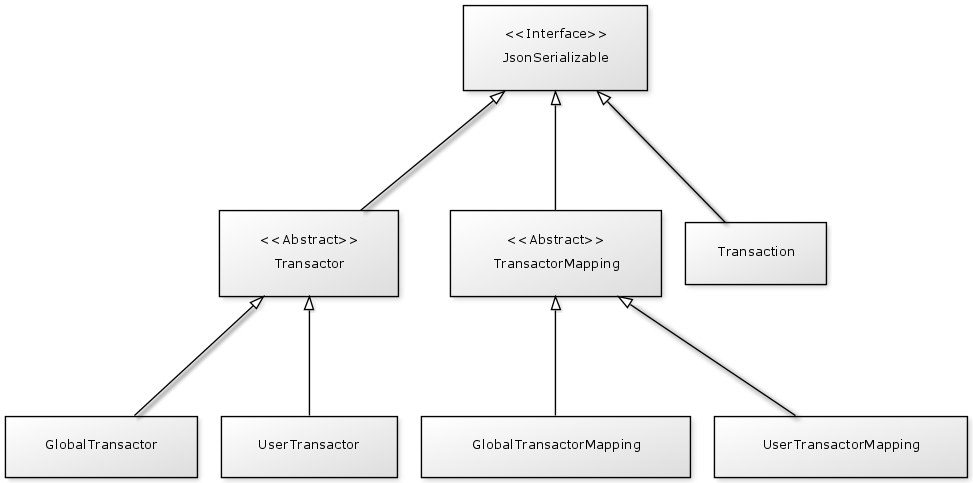
\includegraphics[width=\textwidth]{implementation/json-serializable}
    \caption{Inheritance diagram of JsonSerializable objects}
    \label{fig:mapping-inheritance-diagram}
    
    \begin{comment}
[<<Interface>> JsonSerializable]^-[<<Abstract>> Transactor]
[<<Interface>> JsonSerializable]^-[<<Abstract>> TransactorMapping]
[<<Interface>> JsonSerializable]^-[Transaction]
[<<Abstract>> TransactorMapping]^-[UserTransactorMapping]
[<<Abstract>> TransactorMapping]^-[GlobalTransactorMapping]
[<<Abstract>> Transactor]^-[UserTransactor]
[<<Abstract>> Transactor]^-[GlobalTransactor]
    \end{comment}
\end{figure}

\subsubsection{The Suggestions} \label{sec:suggestionimplementation}
The suggestions are made by searching for known global mappings, user mappings, global transactors and user transactors\footnote{In the order of preference} that are similar to the reference name a suggestion is being made for. This is done using the Natural Language Full-Text Search functions provided by MySQL. These functions, including \inlinesql$MATCH$, use a Vector Space Model to rank the relevance of a field relative to the input and signify this relevance using a decimal number, which means it can be treated as a standard field by the database and used to order the results.  \parencite{mysql2014searches}. 

When searching for suggestions the application finds the five most relevant mappings or transactors, according to full text search, loads those objects from the database using the ORM. As the ORM tool uses doesn't have support for full text search a raw SQL query was written that uses PDO's\footnote{PHP Data Objects extension for accessing databases} prepared statements functionality to send the parameters to the database server, avoiding SQL injection. The query for finding global transactor mappings as part of the \inlinephp{GetCloseTransactorMappings} method in the GlobalTransactorMappingPeer class is shown in Fig. \ref{fig:sql-match-query}, where \inlinesql{:identifier} is replaced by the server with the passed parameters.

\begin{figure}
\centering
\lstset{style=phpcolor}
\begin{lstlisting}[language=sql]
SELECT *, MATCH(:nameColumn) AGAINST (:name) AS 'score'
FROM :tableName
	WHERE :transactorID IS NOT NULL
	HAVING `score` > :minScore OR :nameColumn = :name
ORDER BY `score` DESC
LIMIT 5
\end{lstlisting}
\caption{SQL query selecting similar mappings using PDO}
\label{fig:sql-match-query}
\end{figure}

\section{Prediction}
The key difficulty of implementing the prediction functionality was designing a data structure that allowed predictions to be read by column or by row in order to generate the table output shown in Fig. \ref{fig:imp-categories-overview}. Ordinarily a multidimensional array or a dictionary of dictionaries would be used, however in this case it must be possible to access the data by subcategory as well as by month or date.
%
In order to allow accessing the data by month, category and subcategory as well as being able to generate totals the data structure shown in Fig. \ref{fig:prediction-inheritance-diagram} was used. The TransactionCollection interface defines three methods, \inlinephp{getTotalValue()}, \inlinephp{getTransactions()} and \inlinephp{addTransaction(Transaction)}. Using this interface means that each level of the data structure can be treated in exactly the same way and has the advantage that the entire PersonalBudget object can be passed to the template engine with no controller logic or pre-calculation. Transactions are added to the PersonalBudget object and at each layer of the data structure organised into the correct collection automatically. When getting the transactions from any collection, the object calls the get \inlinephp{getTransactions()} method on any sub-collection instances it holds and returns an intersection of the results.

\begin{figure}[h]
    \centering
    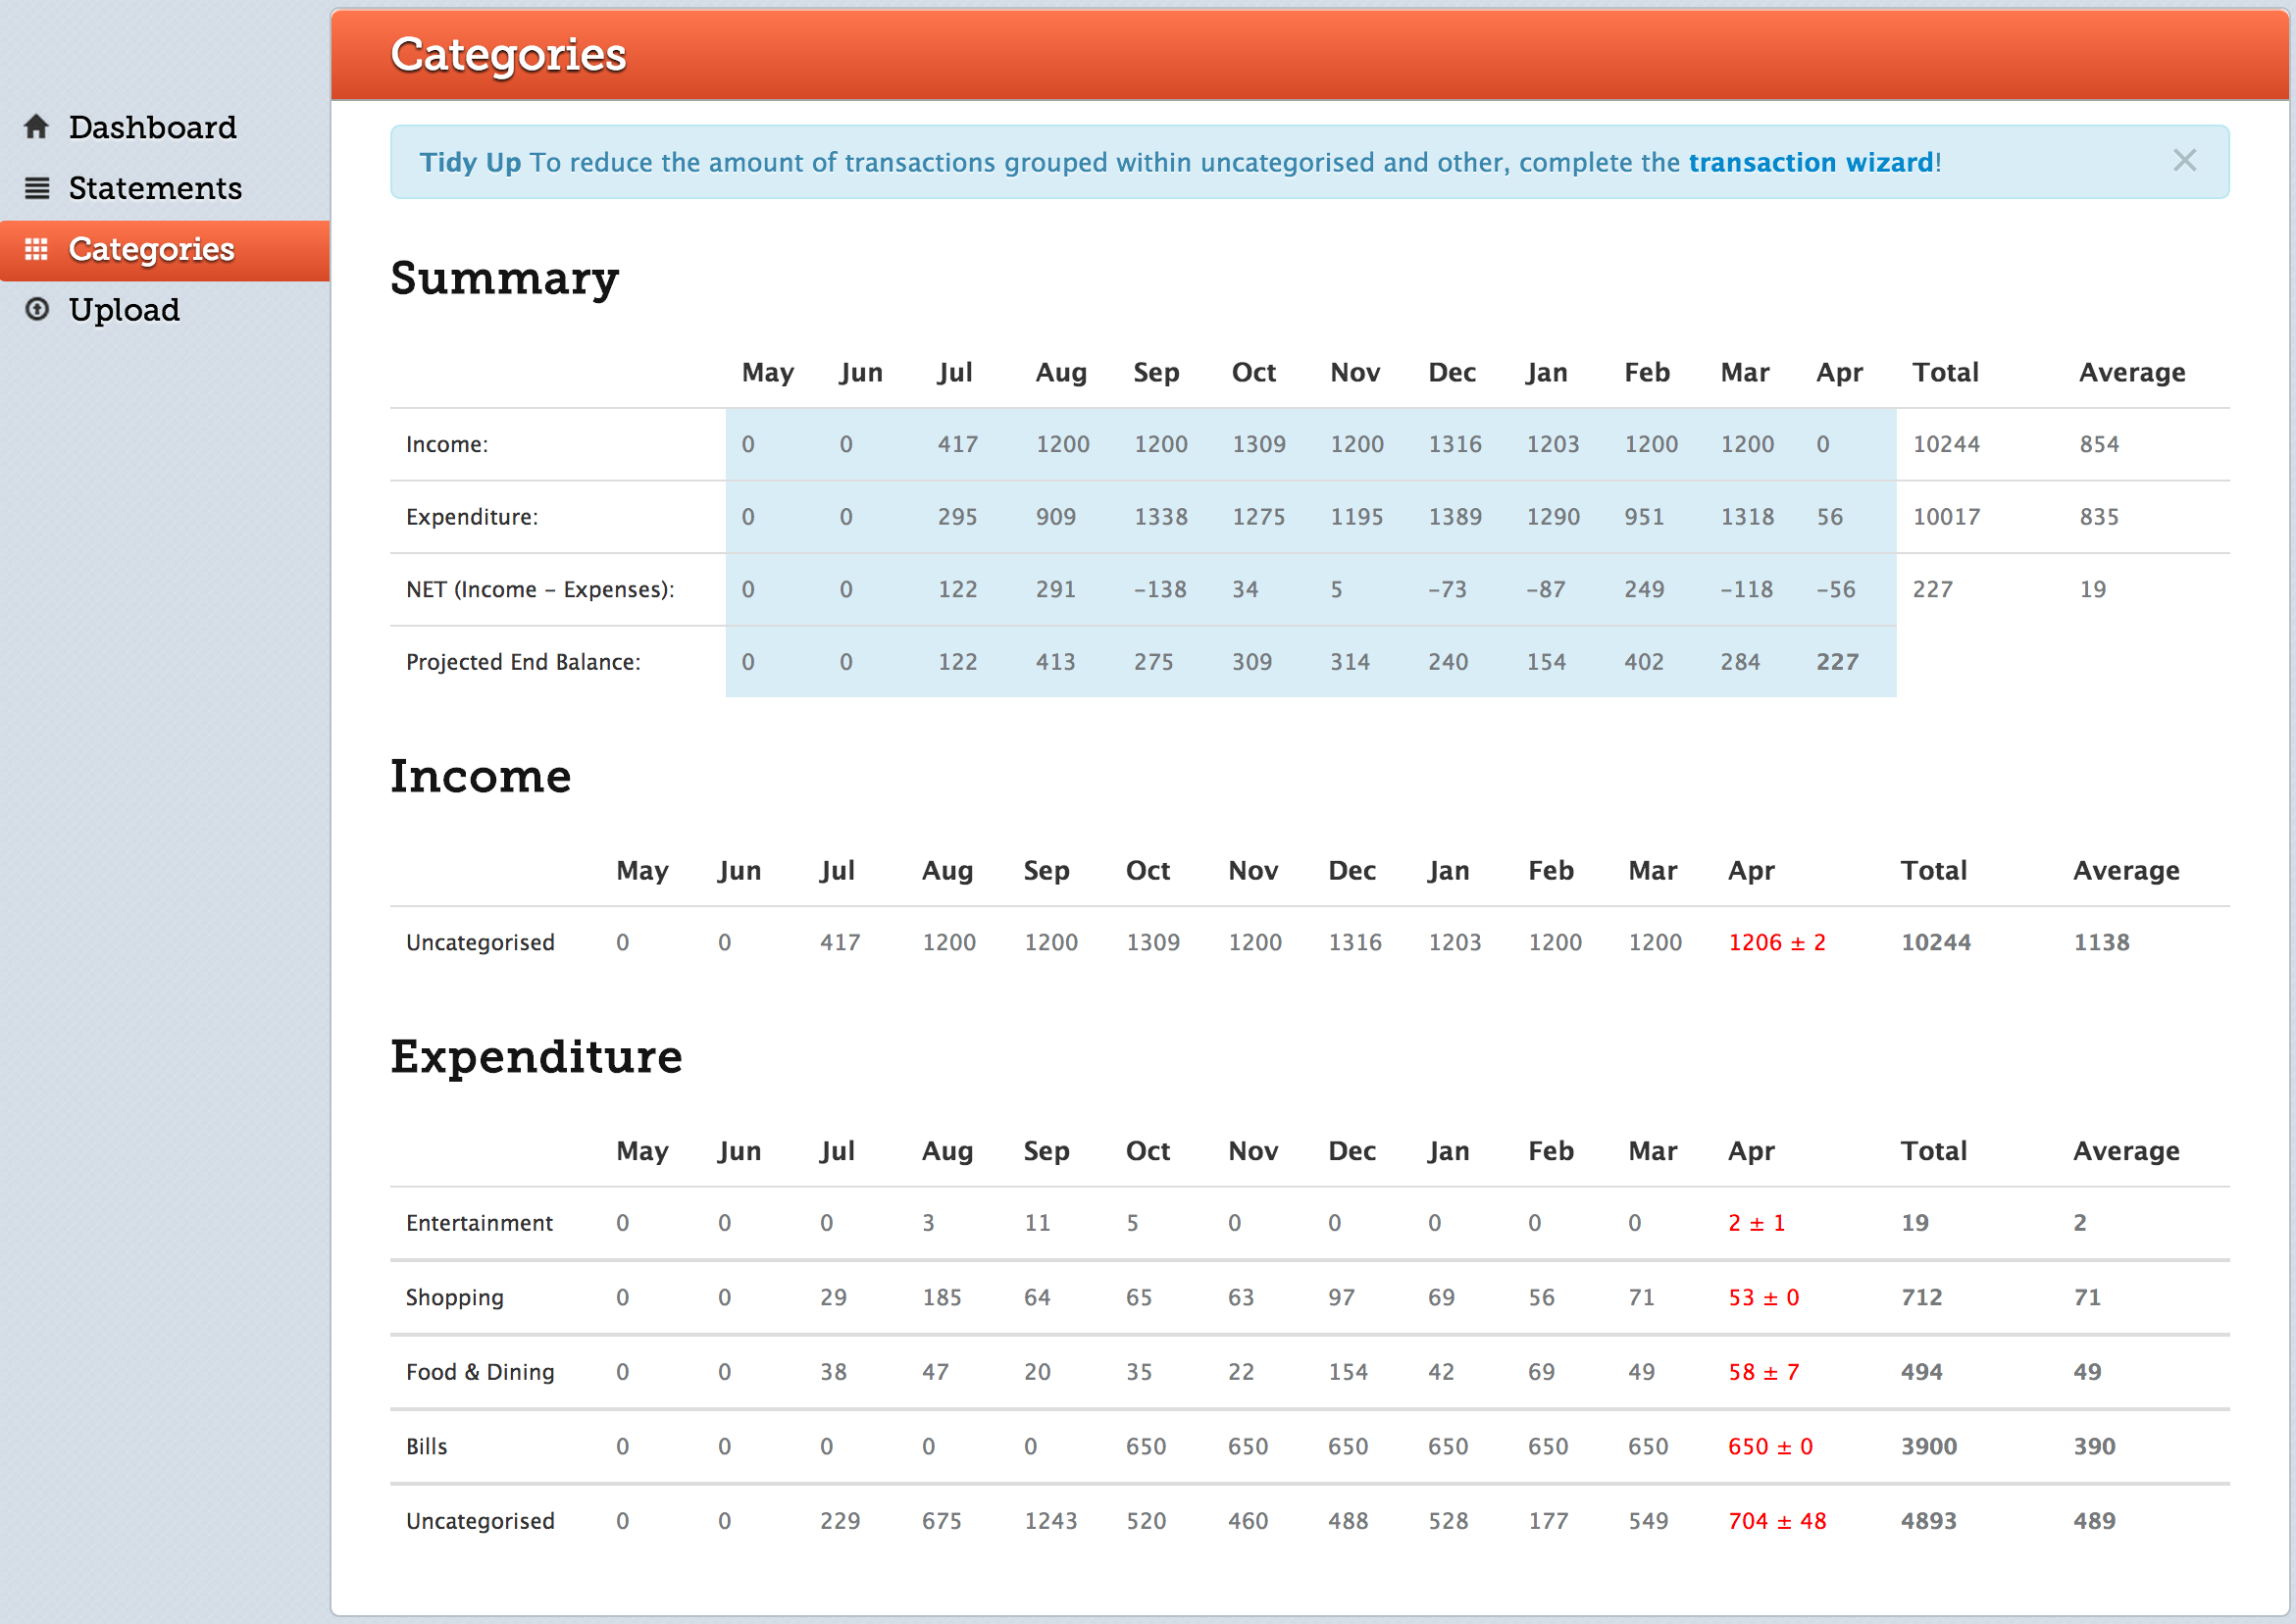
\includegraphics[width=0.75\textwidth]{implementation/categories-overview-2}
    \caption{The budget overview screen where predictions are in red}
    \label{fig:imp-categories-overview}
\end{figure}

\begin{figure}[h]
    \centering
    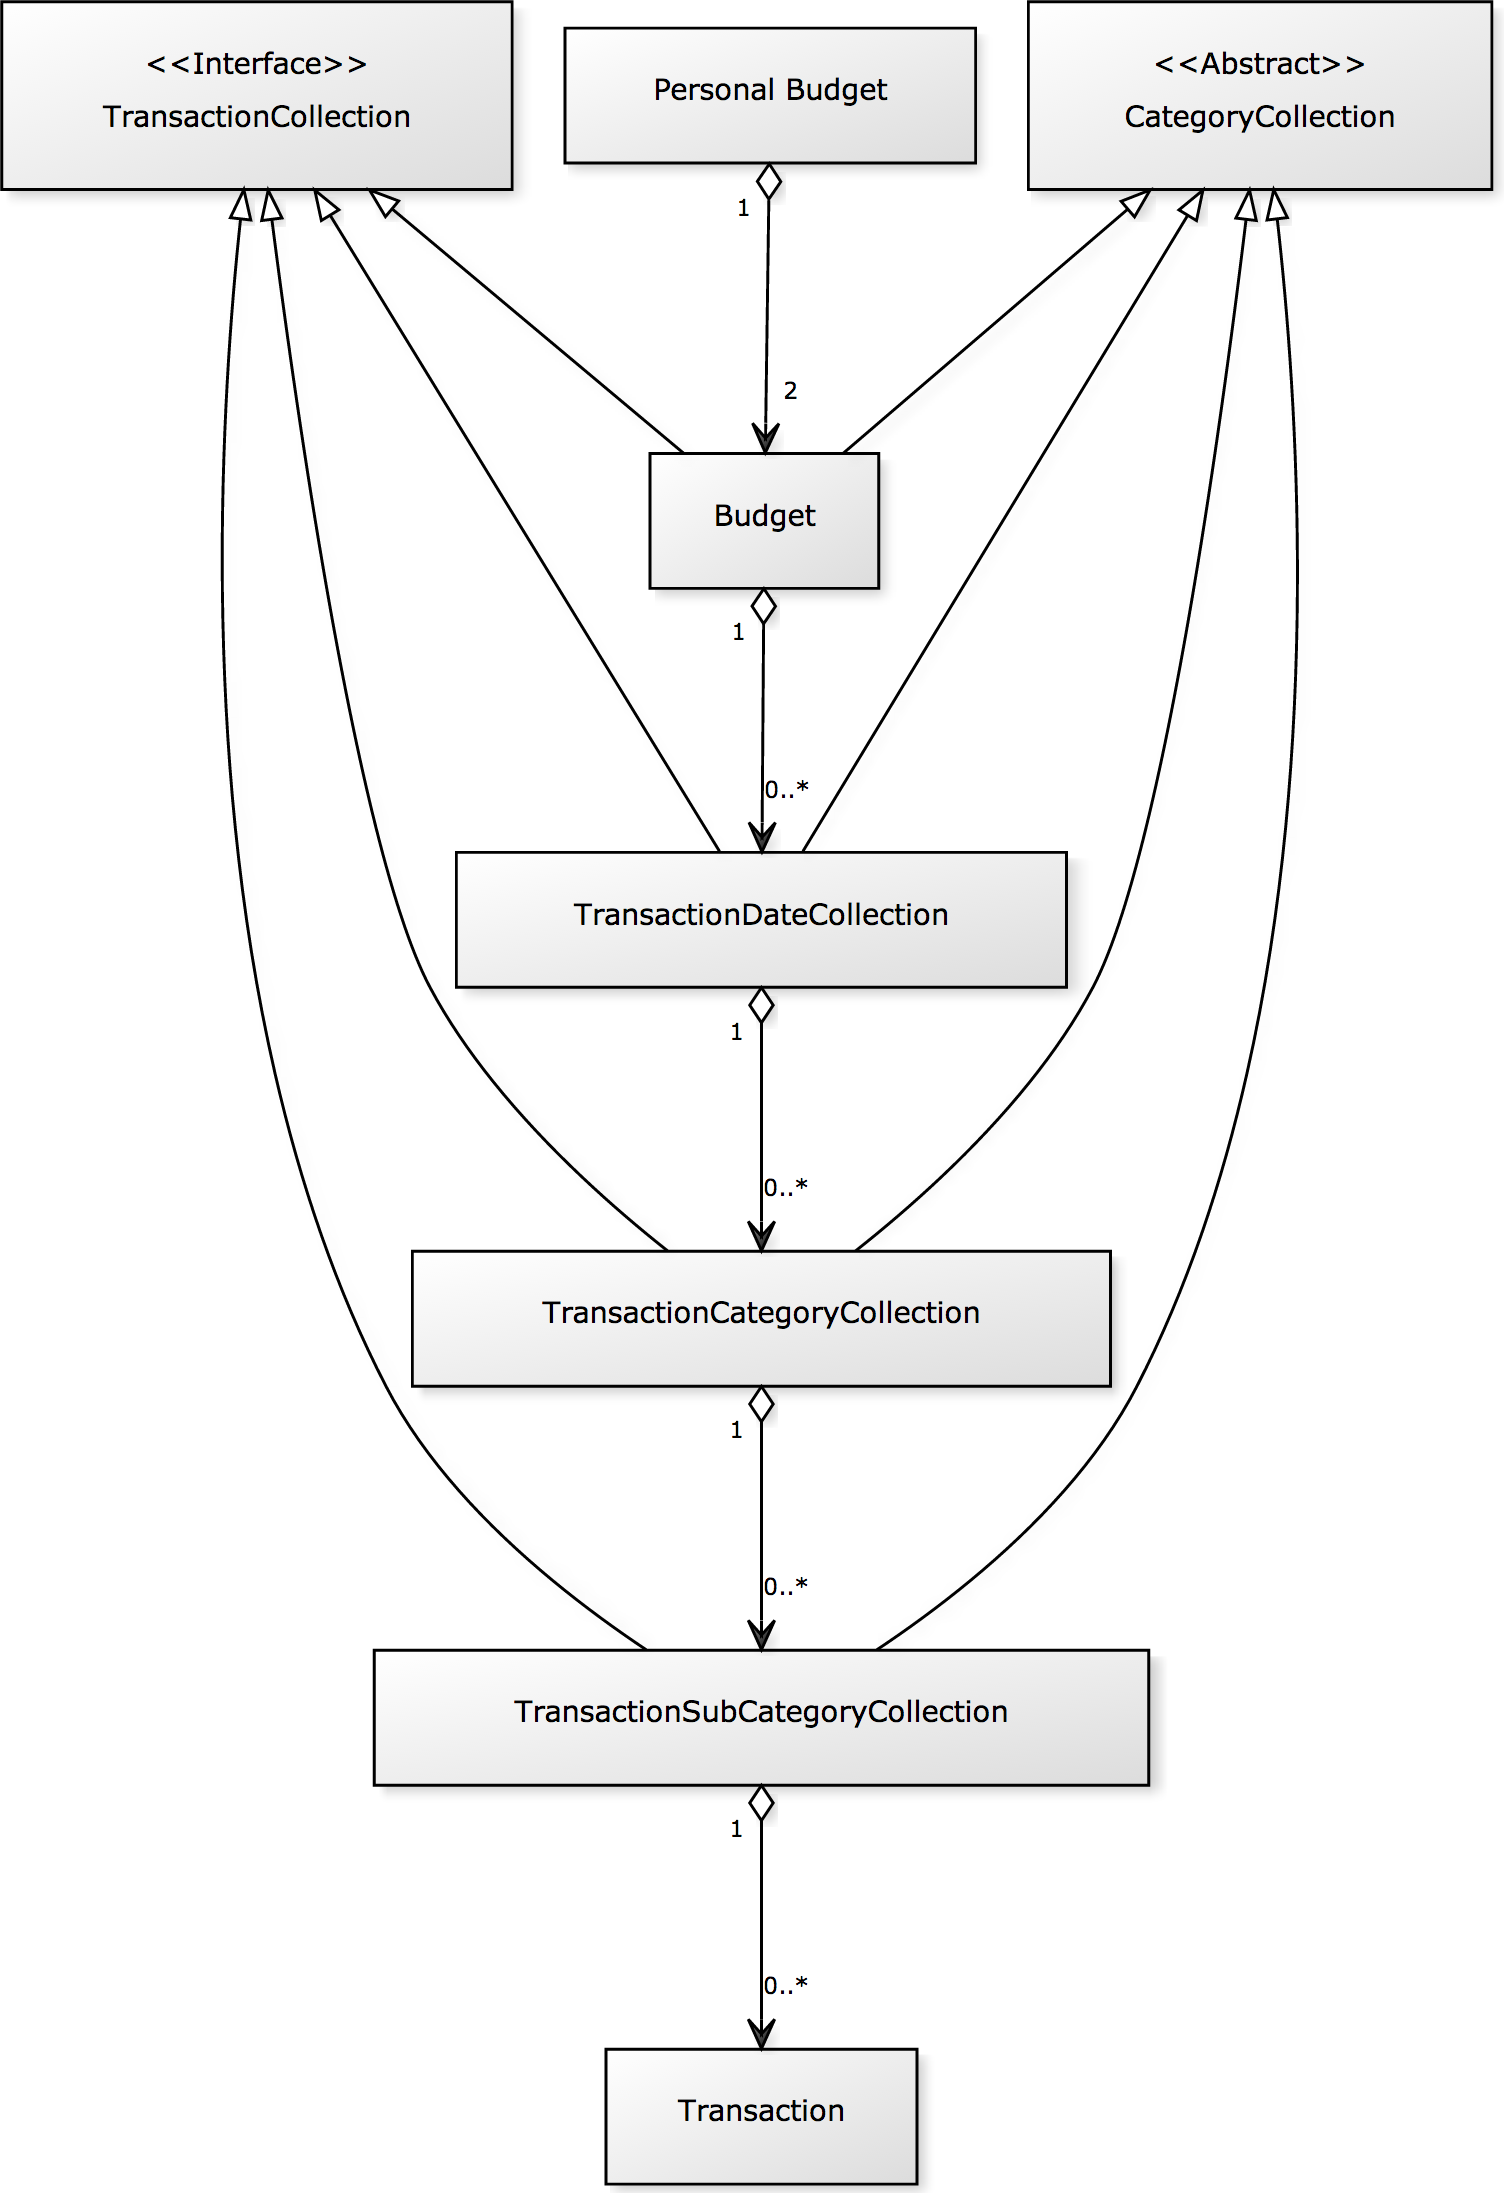
\includegraphics[width=0.75\textwidth]{implementation/mapping-inheritance-diagram}
    \caption{Storing a Personal Budget by date and category}
    \label{fig:prediction-inheritance-diagram}
    
    \begin{comment}
[PersonalBudget]<>1-2>[Budget]
[<<Abstract>> CategoryCollection]^-[Budget]
[<<Interface>>;TransactionCollection]^-[Budget]
[<<Abstract>>;CategoryCollection]^-[TransactionDateCollection]
[<<Interface>>;TransactionCollection]^-[TransactionDateCollection]
[Budget]<>1-0..*>[TransactionDateCollection]
[<<Abstract>>;CategoryCollection]^-[TransactionCategoryCollection]
[<<Interface>>;TransactionCollection]^-[TransactionCategoryCollection]
[TransactionDateCollection]<>1-0..*>[TransactionCategoryCollection]
[<<Abstract>>;CategoryCollection]^-[TransactionSubCategoryCollection]
[<<Interface>>;TransactionCollection]^-[TransactionSubCategoryCollection]
[TransactionCategoryCollection]<>1-0..*>[TransactionSubCategoryCollection]
[TransactionSubCategoryCollection]<>1-0..*>[Transaction]
    \end{comment}
\end{figure}

The Budget object (representing expenditure or income) provides the \inlinephp{getCategoryPrediction()} method which takes a month and a category and returns the systems prediction for that month. It's this method that builds and samples from the Markov Chain Models, calculates the Weighted Arithmetic Mean, and chooses the Weighting Model which provides the least absolute error for the historical data in order to make the prediction. The class also calculates the confidence interval which is displayed in the UI.

The logic for these steps is split into separate classes to improve cohesion and the overall process is shown in Fig \ref{fig:prediction-activity}. \todo{Fix}

\begin{figure}[h]
    \centering
    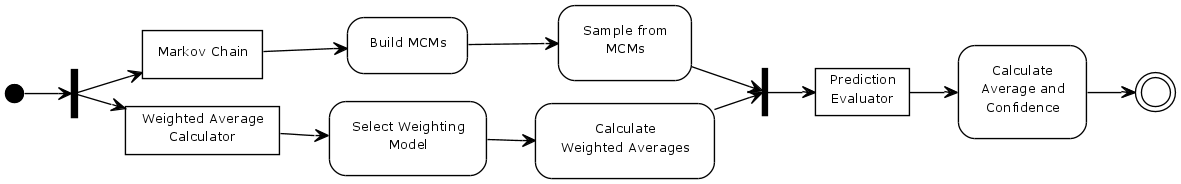
\includegraphics[width=\textwidth]{implementation/prediction-activity}
    \caption{System activity diagram when making a prediction}
    \label{fig:prediction-activity}
    
    \begin{comment}
(start)->|a|
|a|->[Markov Chain]->(Build MCMs)->(Sample from MCMs)->|b|
|a|->[Weighted Average Calculator]->(Select Weighting Model)->(Calculate Weighted Averages)->|b|
|b|->[Prediction Evaluator]->(Calculate Average and Confidence)->(end)
    \end{comment}
\end{figure}

In order to build the Markov Chain Model the TransactionMarkovChain object takes an list of Transaction objects and counts the months where a transaction occurs, storing this in an associative array. This matrix is read to generate a transition table which represents the amount of time a transaction as transitioned from occurring to not occurring and visa-versa. This transition table can be converted to a transition matrix which represents the probability of such a transition occurring. An example transition table and matrix for a one of purchase are shown in Table \ref{table:transition-matrix} and \ref{table:transition-table}.
%
Considering whether or not a transaction occurred in the previous month, a sample is taken from the matrix. For example, if example event occurred last month for the probability of the event occurring next month given that it occurred last month is $0.00$ and so there is a 0\% chance the system will predict the event will occur next month. This process of sampling is repeated up to $10,000$ times for each transaction in under one second and the list of predictions is returned to the Budget class.


\begin{table}[!htb]
  \centering
    \begin{tabular}{lll}
    \#           & Didn't Occur & Occurred \\
    Didn't Occur & 10           & 1       \\
    Occurred     & 1            & 0      
    \end{tabular}
    \caption{Transition table for a one off purchase}
    \label{table:transition-table} 
\end{table}

\begin{table}[!htb]
  \centering
    \begin{tabular}{lll}
    \#           & Didn't Occur & Occurred \\
    Didn't Occur & 0.91         & 0.09       \\
    Occurred     & 1.00         & 0.00     
    \end{tabular}
    \caption{Transition matrix for a one off purchase}
    \label{table:transition-matrix}
   
\end{table}

Having decided whether or not a transaction will occur the Budget class uses an instance of \inlinephp{TransactionWeightedAverageCalculator} to estimate how much money would be transferred if a transaction occurs. The weighted average calculator takes a list of Transaction objects and returns an associative array containing the weighted average for each transactor. To calculate the weighted averages the calculator first selects the best weighting model for the users spending pattern in the specified category and uses the selected function to calculated the averages for each transactor in the category. \todo{Needs fixing}.

Combining the output of the MCM's and the weighted average calculator the produces the systems expenditure prediction for the considered category, Table \ref{table:predictions-combined}. This is calculated for each sample taken from the MCM and the results are passed to an instance of the PredictionEvaluator to produce an average and confidence interval, which is ultimately displayed on the UI.

\begin{table}[h]
\centering
\begin{tabular}{llll}
Transactor  & Prediction & Weighted Average                   & Total        \\
Tesco       & No         & £33                                & £0           \\
Sainsbury's & Yes        & £65                                & £65          \\
Amazon      & No         & £3                                 & £0           \\
Argos       & No         & £17                                & £0           \\
            &            & \multicolumn{1}{r}{\textbf{Total}} & \textbf{£65}
\end{tabular}

\caption{Combination of the samples from the MCM and the weighted averages}
\label{table:predictions-combined}
\end{table}

\section[Security]{Security Considerations}
The security considerations outlined in section \ref{section:security}, were implemented throughout the project including site-wide SSL, password entropy requirements, password salting and hashing and personal identifiable information encryption. In addition the application implements additional protection against account hijacking and login throttling to reduce the overall effectiveness of brute force attacks. 

An overview of the techniques used during login and on every page request is shown in Fig. \ref{fig:login-security} and \ref{fig:page-request-security}.

\begin{figure}[h]
    \centering
    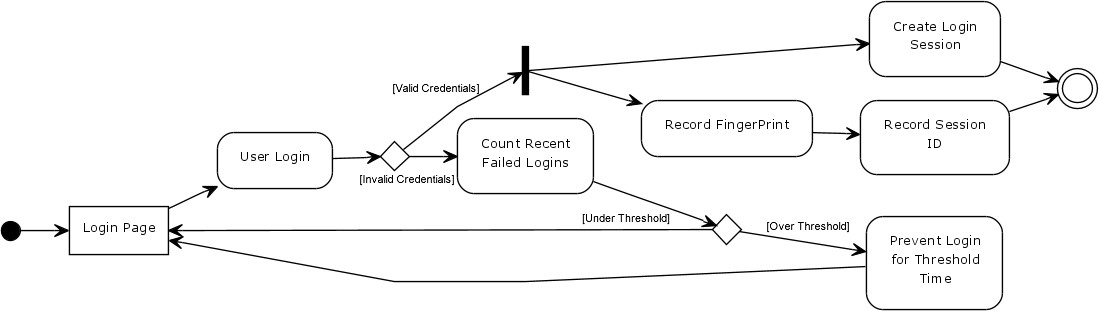
\includegraphics[width=\textwidth]{implementation/login-security}
    \caption{Steps performed during a user login}
    \label{fig:login-security}
    
    \begin{comment}
(start)->[Login Page]->(User Login)-><a>
<a>->|b|
<a>->(Count Recent Failed Logins)-><d>
<d>->(Prevent Login for Threshold Time)->[Login Page]
<d>->[Login Page]
|b|->(Create Login Session)->(end)
|b|->(Record FingerPrint)->(Record Session ID)->(end)
    \end{comment}
\end{figure}

\begin{figure}[h]
    \centering
    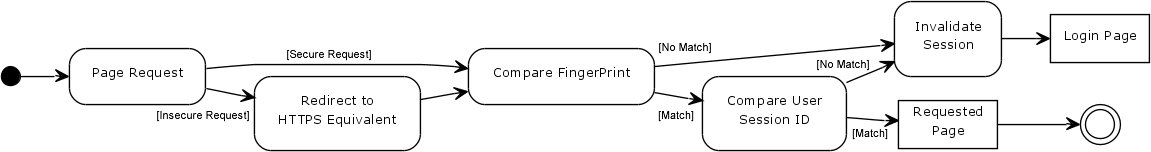
\includegraphics[width=\textwidth]{implementation/page-request-security}
    \caption{Steps performed during every page load request}
    \label{fig:page-request-security}
    
    \begin{comment}
(start)->(Page Request)
(Page Request)->(Compare FingerPrint)
(Page Request)->(Redirect to HTTPS Equivalent)->(Compare FingerPrint)
(Compare FingerPrint)->(Compare User Session ID)
(Compare FingerPrint)->(Invalidate Session)->[Login Page]
(Compare User Session ID)->(Invalidate Session)
(Compare User Session ID)->[Requested Page]->(end)
    \end{comment}
\end{figure}


\subsection{Account Hijacking}
The users session\footnote{Stored server side} identified by the session ID in the users cookie,  includes a fingerprint of the users browser user agent, an additional user session identifier, the last time they performed an action as well as the users ID, these are validated on every page load and if incorrect the session is invalidated, to prevent further use, and the user is logged out.


The fingerprint and session identifier provide an additional layer of protection against account hijacking and recording the last action time means that if a user leaves their computer idle or forgets to logout their session cannot be used after a certain amount of time has passed.

The user session identifier is generated each time a user logs in, and stored in their user record. On each page load the recorded identifier is compared to the current one found in the users session, if they don't match the user must have an old session and their session is no longer valid. This prevents use of an old session if the user has logged in elsewhere, such as logging in from another computer or mobile device.

Fingerprinting relies on the user agent string (UAS) which sent in the HTTP headers to the remote server by the users browser and contains information including their current browser version and operating system, example UAS' are shown in Fig. \ref{fig:useragentstring}. It's important to note that although the string can be manipulated using a browser extensions or modifying to string sent in the HTTP header the average user would not be doing this and for the purposed of purposes of fingerprinting the actual value is not of particular importance, as long as it doesn't change value between requests implying the user is logging in from a different device using the same session (as would be seen during account hijacking).

\begin{figure}
\centering
\begin{subfigure}[a]{\textwidth}
\centering
\texttt{Mozilla/5.0 (Macintosh; Intel Mac OS X 10\_9\_2) AppleWebKit/537.36 (KHTML, like Gecko) Chrome/34.0.1847.131 Safari/537.36}
\caption{Google Chrome running on OS X}
\label{fig:uasforchrome}
\end{subfigure}

\begin{subfigure}[b]{\textwidth}
\centering
\texttt{Mozilla/5.0 (iPad; CPU OS 5\_1 like Mac OS X; en-us) AppleWebKit/534.46 (KHTML, like Gecko) Version/5.1 Mobile/9B176 Safari/7534.48.3}
\caption{ Google Chrome running on OS X}
\end{subfigure}

\begin{subfigure}[c]{\textwidth}
\centering
\texttt{Mozilla/5.0 (compatible; MSIE 10.0; Windows NT 6.1; Trident/6.0)}
\caption{Internet Explorer 10 on Windows 7}
\end{subfigure}

\begin{subfigure}[d]{\textwidth}
\centering
\texttt{Mozilla/5.0 (X11; Ubuntu; Linux x86\_64; rv:24.0) Gecko/20100101 Firefox/24.0}
\caption{Firefox 24 on Linux (Ubuntu)}
\end{subfigure}

\caption{Example User Agent String's}
\label{fig:useragentstring}
\end{figure}

The use of browser fingerprinting to improve session security was suggested and evaluated by \Citeauthor{unger2013fingerprinting} who concluded that the technique was successful in preventing various attacks and hijacking attempts, including XSS and passive sniffing . The paper also demonstrated that FireSheep and WhatsApp Sniffer, discussed in sestion \ref{subsection:account-hijacking} are thwarted by fingerprinting \parencite{unger2013fingerprinting}.

The actual fingerprint taken by the project is similar to that suggested in the paper. Consisting of all of the alphabetic strings found in the UAS concatenated and hashed. Only alphabetic strings are used as the likely-hood of a user updating their browser or operating system is high, particularly considering the automatic update feature which is common in many modern browsers \parencite{google2014autoupdate, firefox2014autoupdate}. The code used to build the browsers fingerprint is shown in Fig. \ref{fig:fingerprinting}.

\begin{figure}
\centering
\begin{lstlisting}[style=phpcolor]
$parts = preg_split('#([^A-z]+)#', $_SERVER['HTTP_USER_AGENT']);
$fingerprint = "";
foreach($parts as $part) {
	if(strlen($part) > 1 || strlen($fingerprint) < 2)
		$fingerprint .= $part;
}
\end{lstlisting}
\caption{Generating a browsers fingerprint using the user agent string}
\label{fig:fingerprinting}
\end{figure}

In a users browser fingerprint changes, their user session id doesn't match the one in the database or the time since their last action is over the threshold their session is both unset\footnote{Frees all session variables \parencite{php2014sessionunset}} and destroyed\footnote{All server side data associated with the session is deleted \parencite{php2014sessiondesroy}} and their which was used to idenfity the session to the server cookie is written over\footnote{Required to `kill the session altogether' \parencite{php2014sessiondesroy}}. This will cause them to be logged out and redirected to the login page, for convenience the page they were previously on is stored and they will return to it on successfully logging in.

Destroying the session in this way means that even if an attacker had successfully performed a session hijack before the destruction occurred the cookie that was stolen is no longer valid and cannot be used for authentication.

\subsection{Brute Force Attacks}

Login throttling was implemented using a database table containing every failed login, the time of the login attempt and for reference the IP address and user the failed login attempt was for.

If a user enters an incorrect username or password an entry is added to the failed login attempt table and the application checks up how many failed password attempts have occurred in the last threshold period\footnote{Defined in a config file to allow easy modification}, see Fig \ref{fig:getThrottlingWaitSeconds}.
%
If the number of attempts is larger than the maximum failed logins per period the user must wait for a few seconds before they can try to login again, that is, all login attempts will fail and the UI will prevent login to avoid users becoming confused.

By enforcing a wait time of only a few seconds  it's likely a normal user would not notice the throttling as they would take a few seconds to login, but an attack would be seriously hampered.
%
The throttling is applied across all user accounts and IP addresses to ensure use of a botnet to send a distributed brute force attack is also very impractical \parencite{stackoverflow2013authentication}.

\begin{figure}
\centering
\begin{lstlisting}[style=phpcolor]
public function getThrottlingWaitSeconds() {
	$throttleSteps = array(60 => 1, 120 => 2, 240 => 3);
	$throttlePeriodMinutes = $this->getConfig()->getThrottlePeriod();
	
	$mostRecent = FailedLoginAttemptPeer::GetMostRecent();		
	if($mostRecent) {
		$mostRecentLoginTimestamp = $mostRecent->getUpdatedAt('U');
		$attemptCount = FailedLoginAttemptPeer::GetCountInLastMinutes($throttlePeriodMinutes);
		
		krsort($throttleSteps);
		foreach($throttleSteps as $attempts => $wait) {
			if($attemptCount > $attempts) {
				return time() - $mostRecentLoginTimestamp - $wait;
			}
		}
	}
	return 0;
}
\end{lstlisting}
\caption{Calculates wait time following a failed login attempt}
\label{fig:getThrottlingWaitSeconds}
\end{figure}

In the future the login throttling system could be extended to take into account the average number of logins per day and automatically adjust the throttling thresholds appropriately.




\begin{comment}
Chapter 5: Results
Results that illustrate how the system designed by you works in practice, and how it is intended to be used, may be presented in this chapter. Screen shots may be useful to illustrate how the software interacts with the user.
\end{comment}

\begin{comment}
Chapter 6: Testing and Evaluation
This chapter should give details of how the system designed and implemented by you was tested. The data and results obtained from this testing whould be presented and consideration be given as to whether or not these results confirm that everything works correctly.

The analysis of test results is very important and some assessment of their significance and quality must be given. Likely sources of error and inaccuracy should be mentioned. Use graphs, bar charts and histograms where appropriate, remembering to label all axes and give scales. The analysis is often done badly, thus sacrificing marks.
\end{comment}

\chapter[Results]{Results and Evaluation}

\plan{Print Screen Step Through of the Main Stuff the Application Does}

\section{System Walk-through}
Below, an overview of the systems behaviour is given following the standard users use case in the form of a walk through. For further exploration of features the application can be found online at \url{https://secure.pezcuckow.com/} where an account can be registered for access.

\begin{figure}
\centering
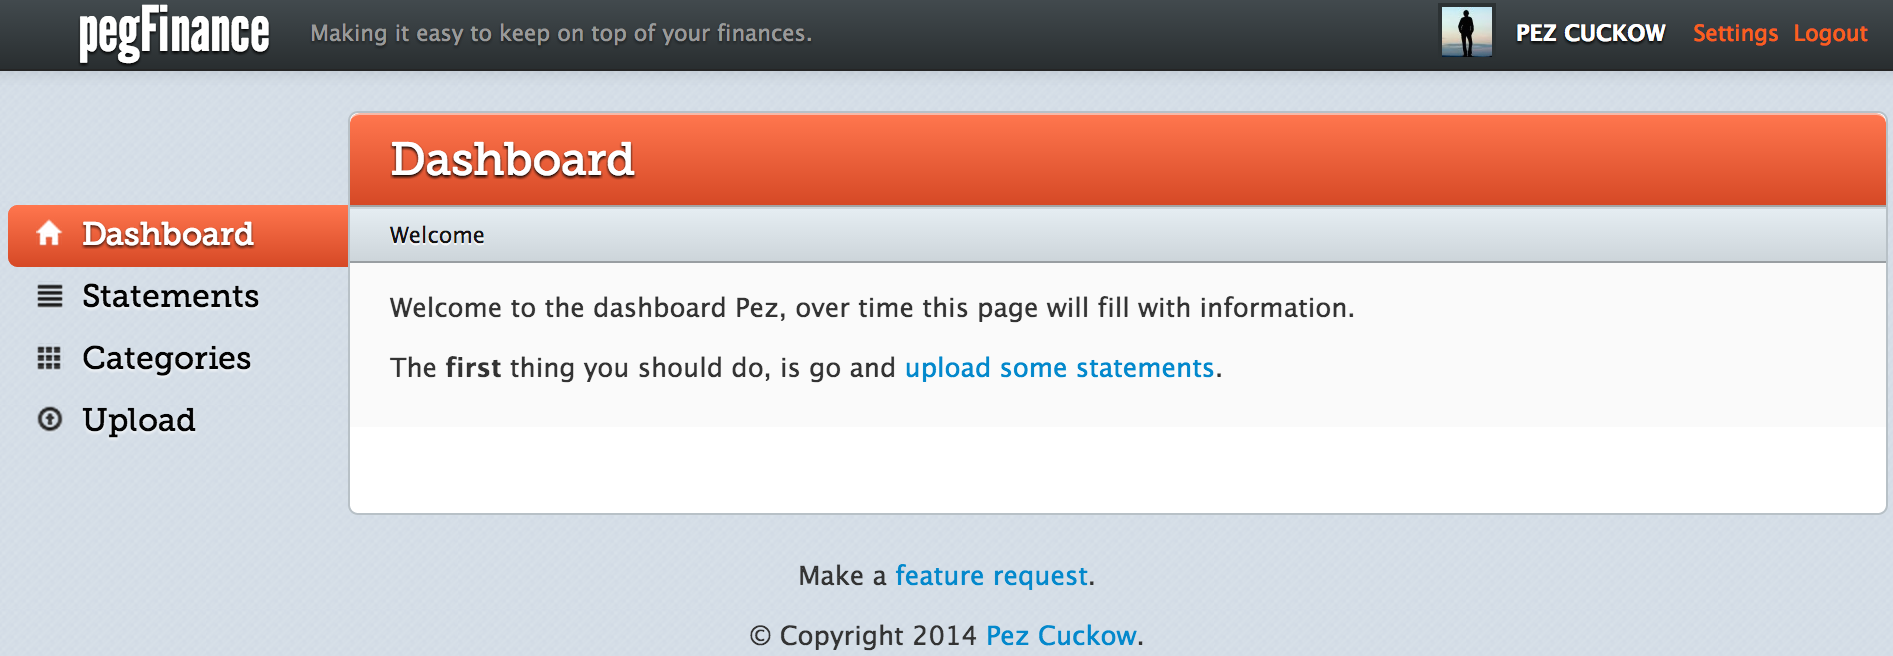
\includegraphics{screenshots/dashboard-empty}
\caption{Empty welcome screen}
\label{fig:welcomescreen}
\end{figure}

Having logged in, the application starts on a welcome screen (Fig. \ref{fig:welcomescreen}} which fills with information over time, for now the system prompts the user to upload a bank statement. The user bar appears at the top of every page which identifies the currently logged in user by name and a avatar pulled using from Gravatar\parencite{gravatar2014avatars}, it provides quick access to the user settings and allows the user to logout.




\subsection{Suggestion Wizard}
\label{subsection:suggestion-wizard-walkthrough}.

\section{Unit Tests}
\plan{Not sure if this fits here!}

\section{Evaluation of the system}
\plan{How did I check that it was working? Testing with personal data, users trying it and running tests of everything}

\missingfigure{Need figures representing accuracy, error, etc}

\section{User feedback}

% SUPR-Q - http://www.measuringusability.com/suprq.php

\section[Responsive Design]{Responsive Web Design}

A key feature of the application is being able to access it at any time from any device, particularly when taking into account the rapid increase in the use of mobile devices.  Interacting with a website on a smartphone or tablet is not the same as interacting using a computer, due to the smaller screen size and use of touch over a mouse.

Forbes reported that 24\% of their 2013 website visits came from mobiles and 13\% from tablets, down from a total of 15\% in 2012. particularly with the high percentage of website visits coming from mobile devices \parencite{steimle2013responsive}.

In order to ensure the project is accessible from a variety of different devices the core UI uses Responsive Web Design (RWD) to layout the website differently depending on the size of the device to ensure an optimal viewing experience.

The differences depending on the device are highlighted in Figs. \ref{fig:responsive-macbook}-\ref{fig:responsive-iphone}.

\begin{figure}[h]
    \centering
    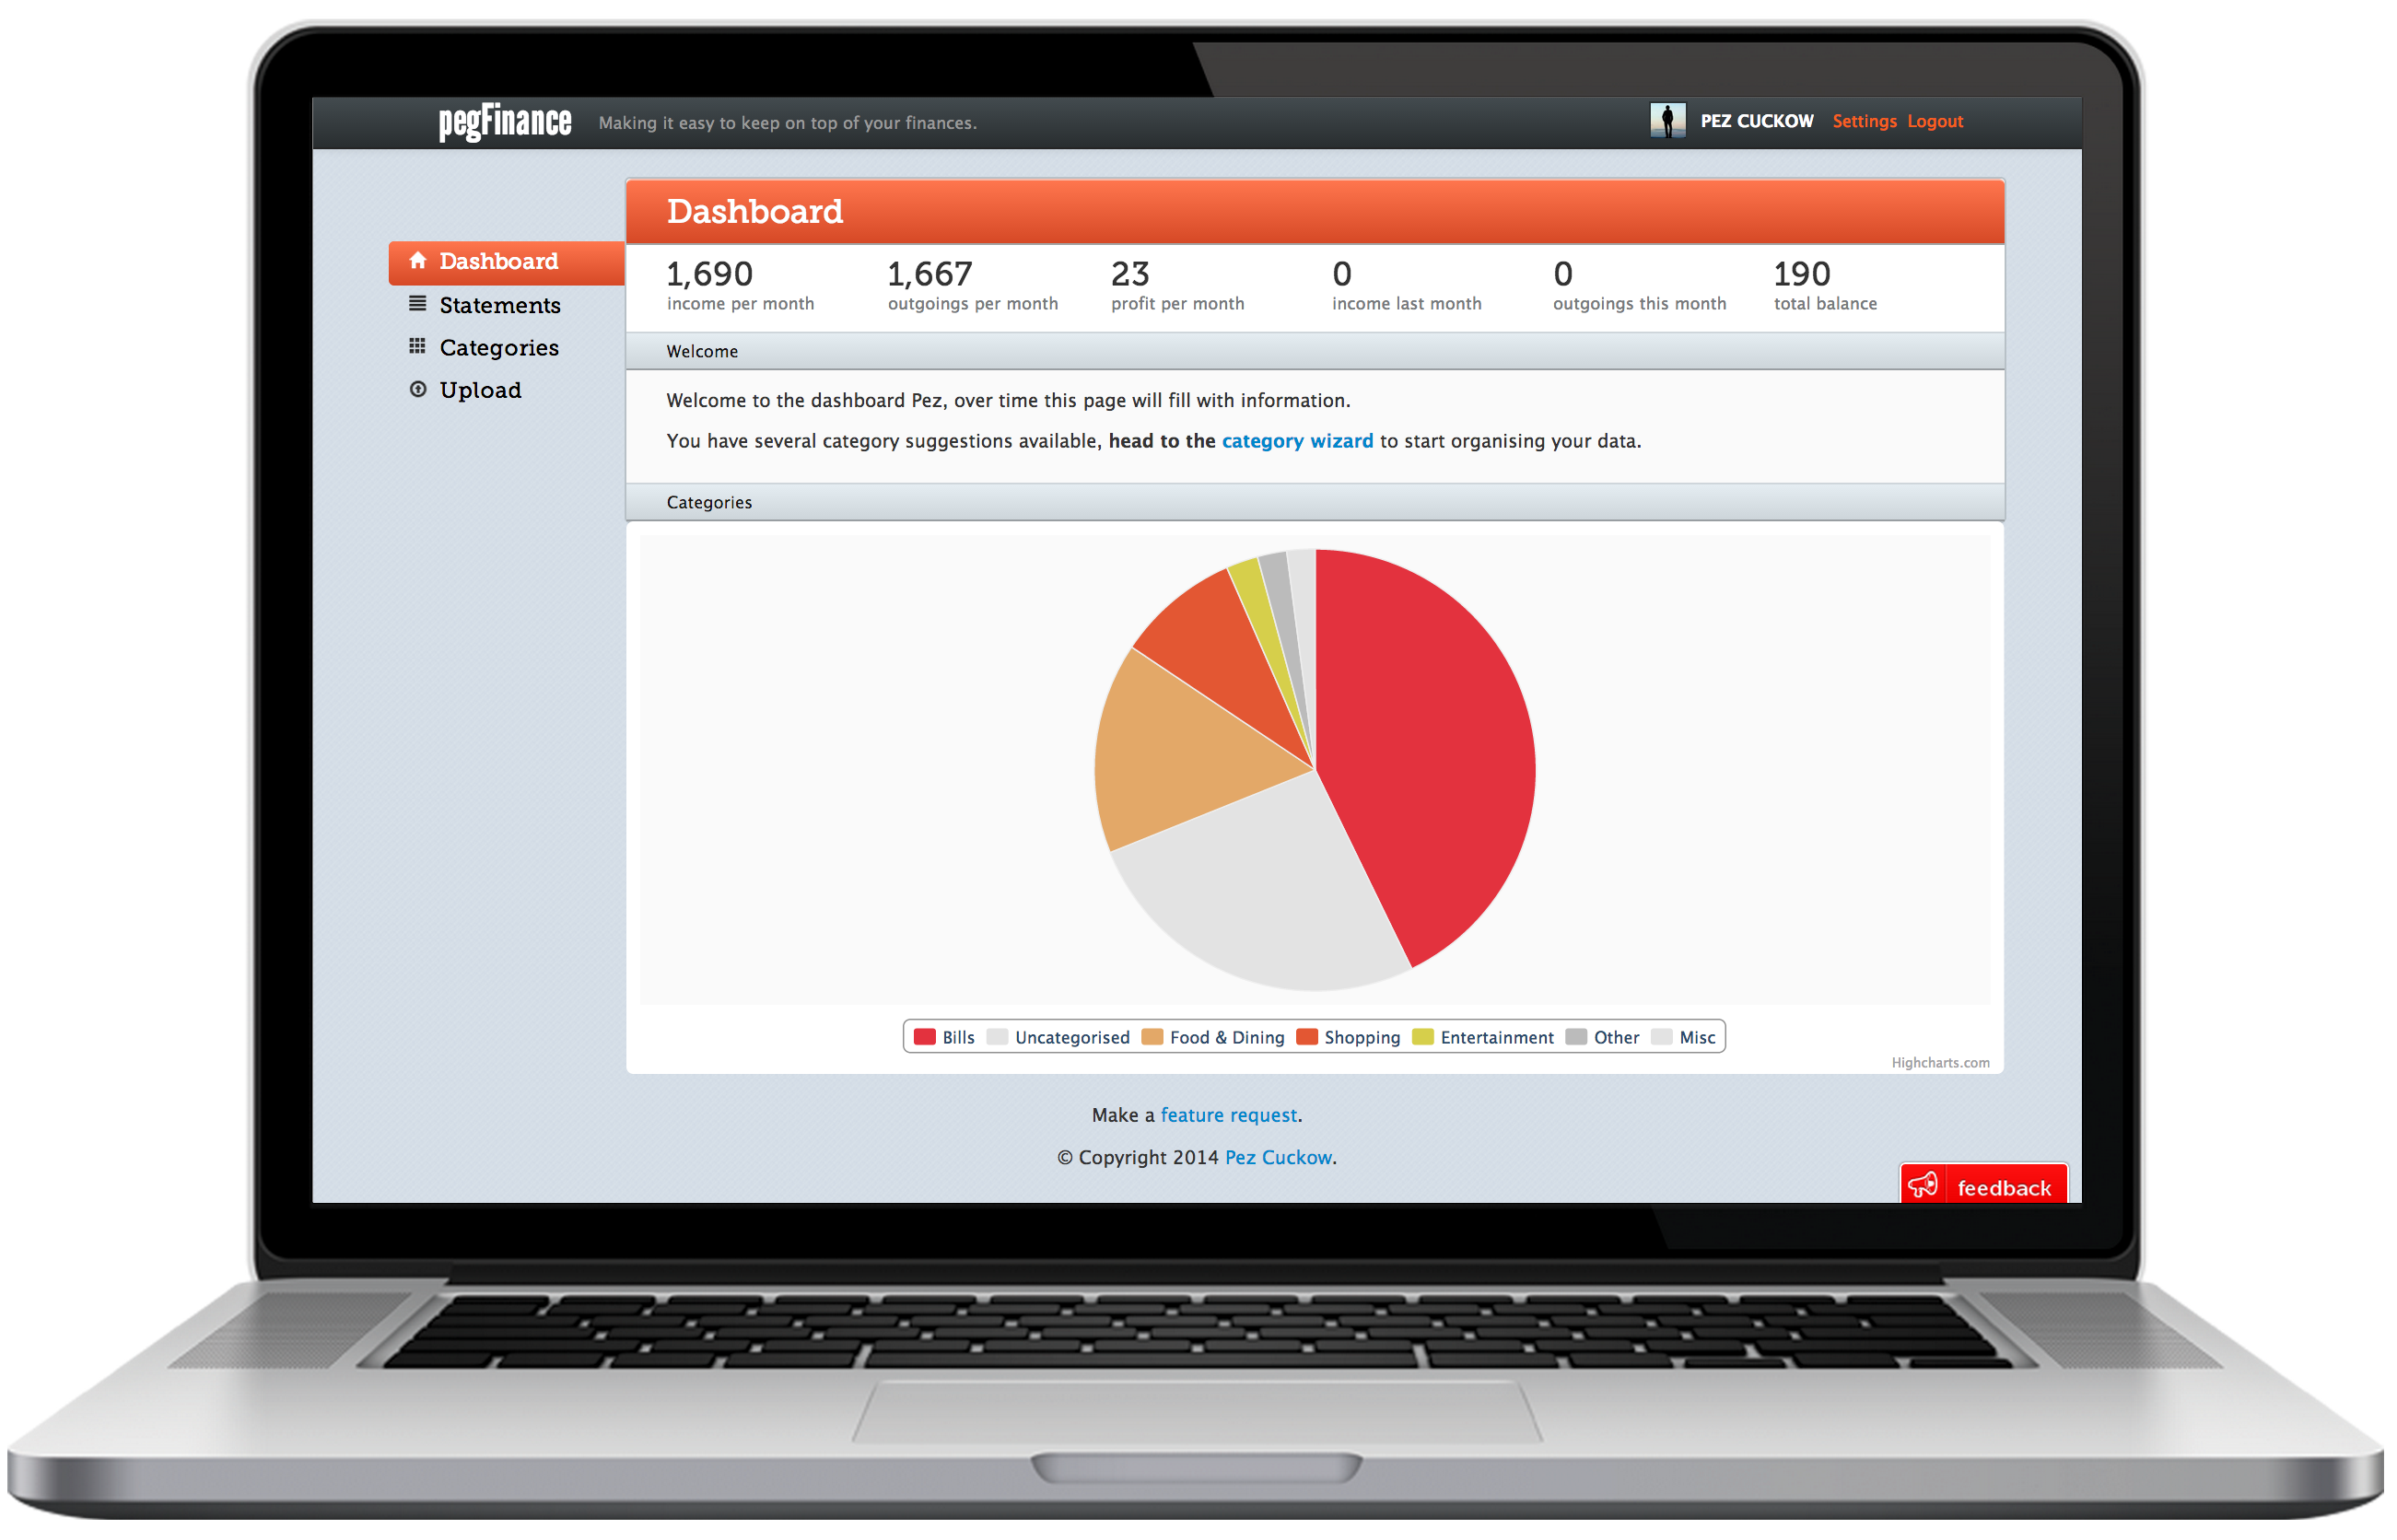
\includegraphics[width=0.8\textwidth]{screenshots/responsive/macbook}
    \caption{Layout on a standard laptop}
    \label{fig:responsive-macbook}
\end{figure}

\begin{figure}[h]
    \centering
    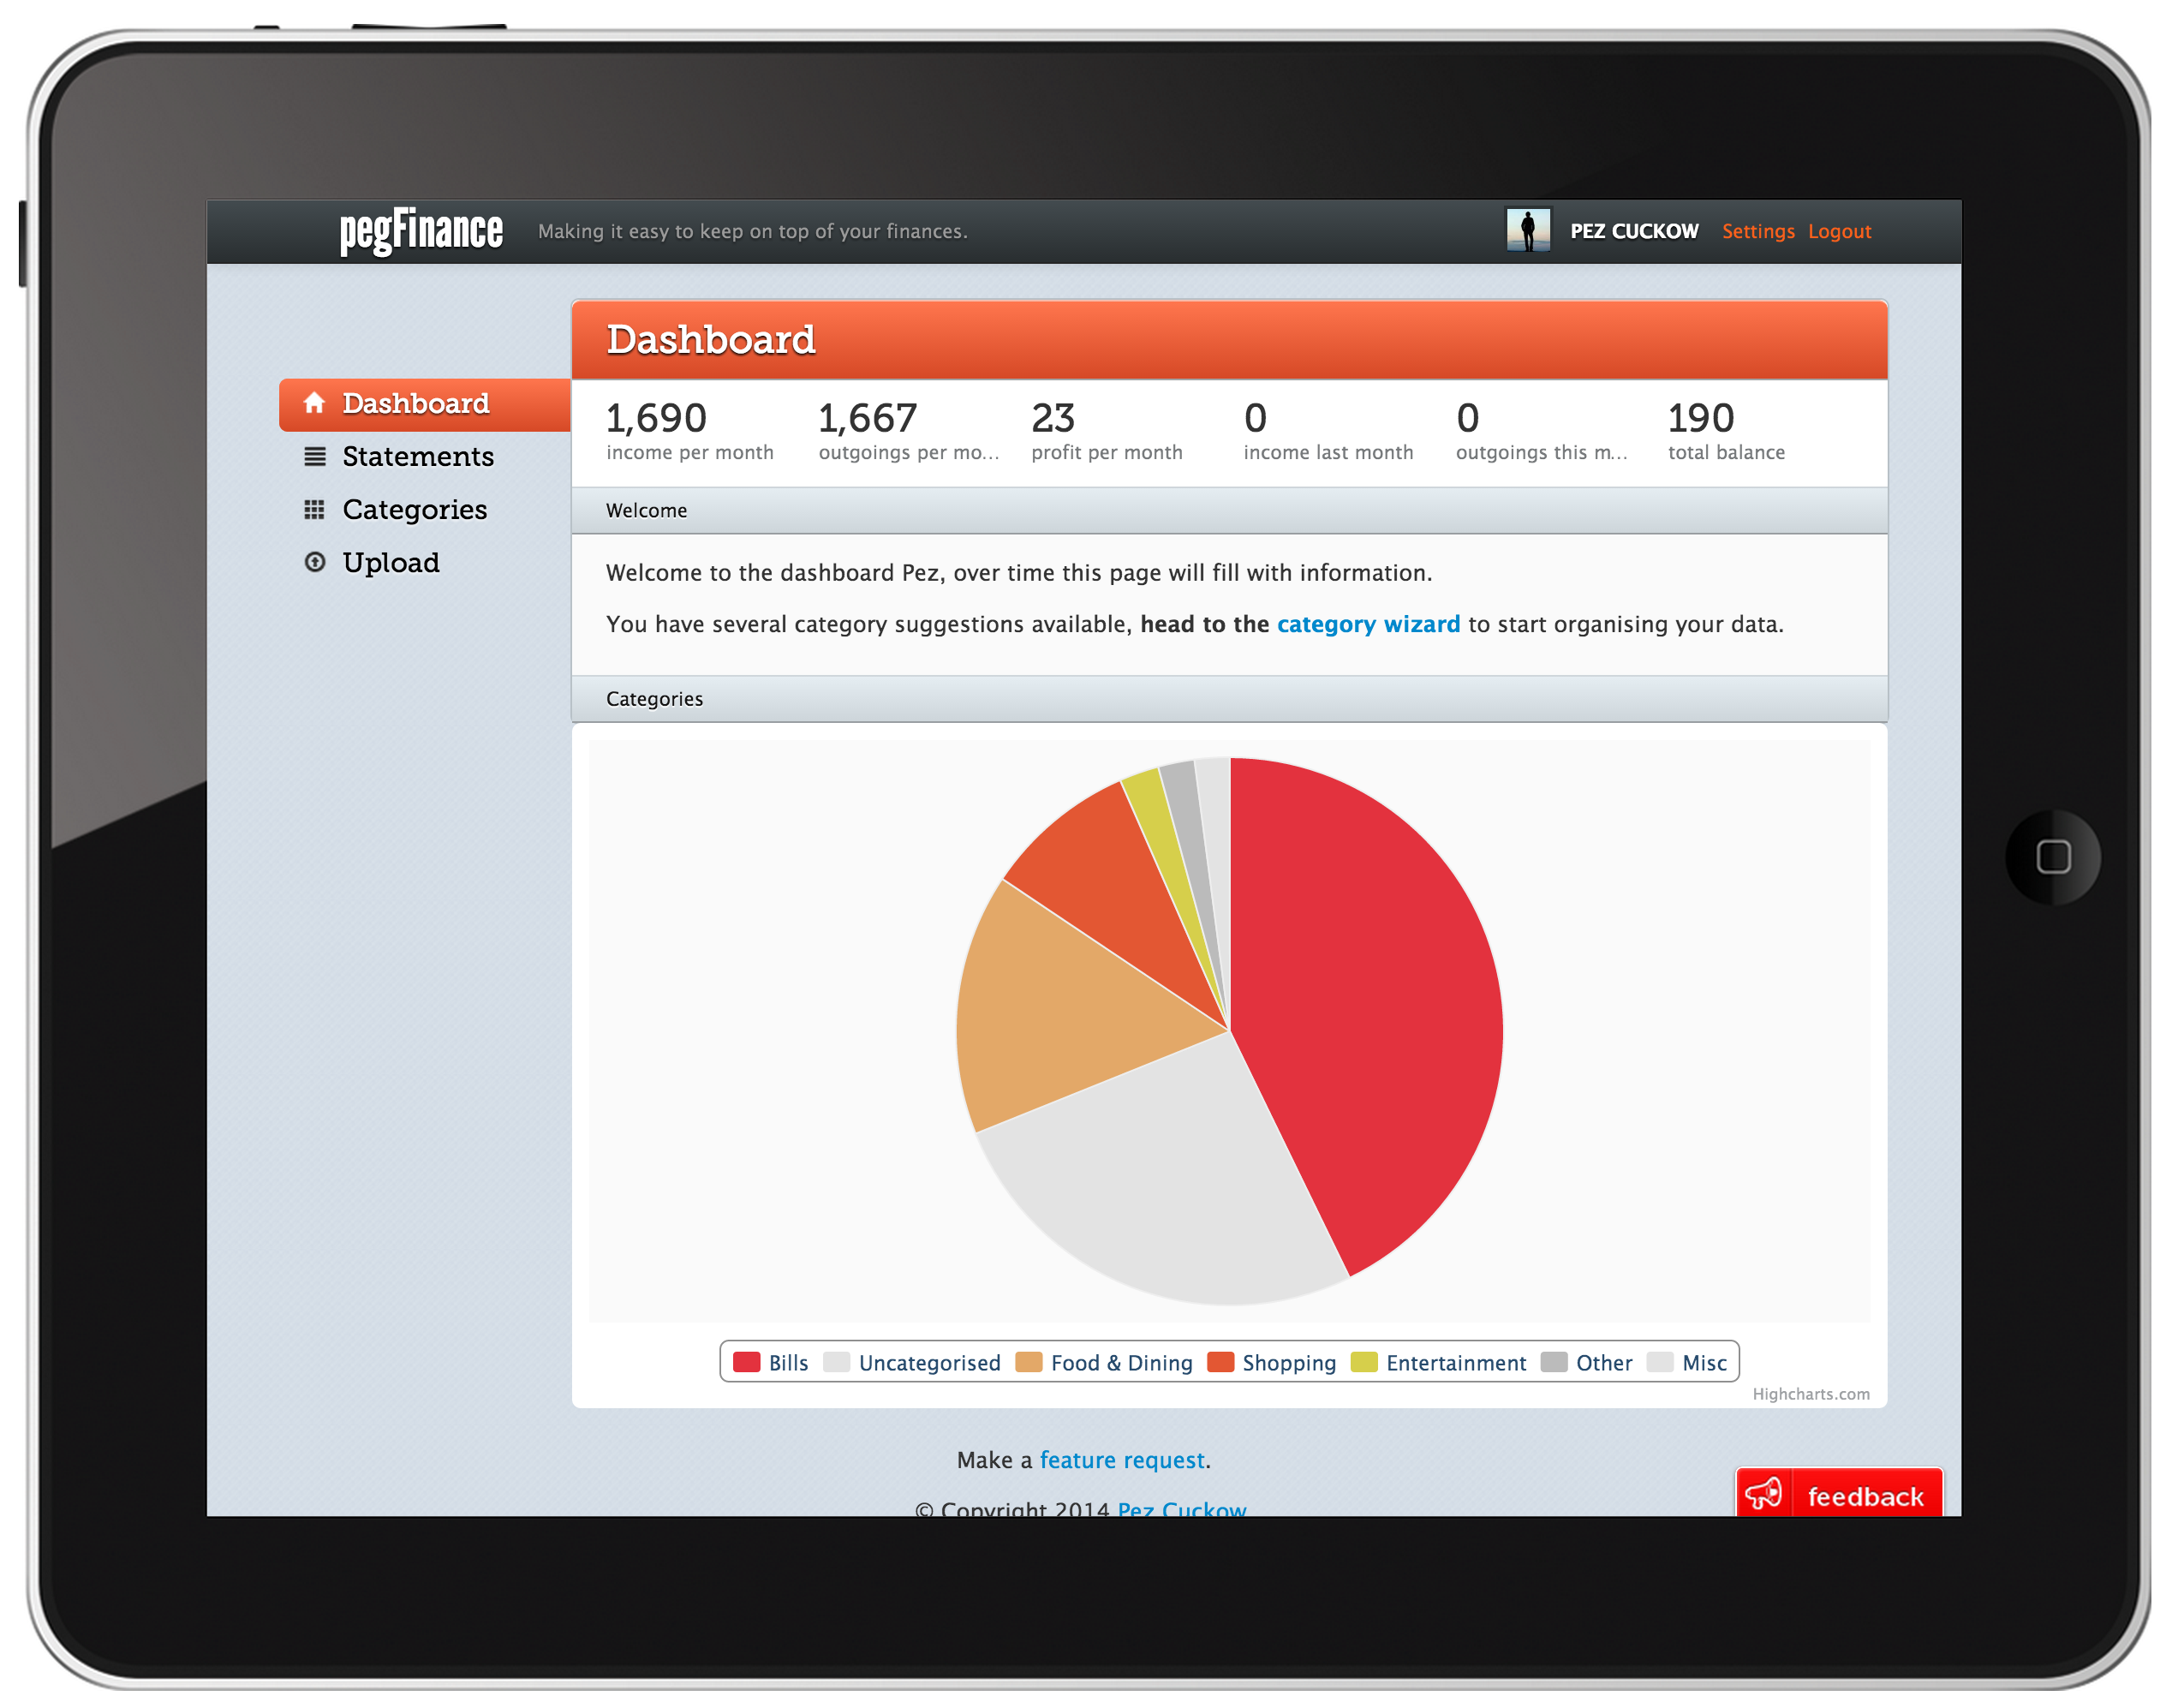
\includegraphics[width=0.8\textwidth]{screenshots/responsive/ipad-sideways}
    \caption{Layout on a tablet in landscape}
    \label{fig:responsive-ipad}
\end{figure}

\begin{figure}[h]
    \centering
    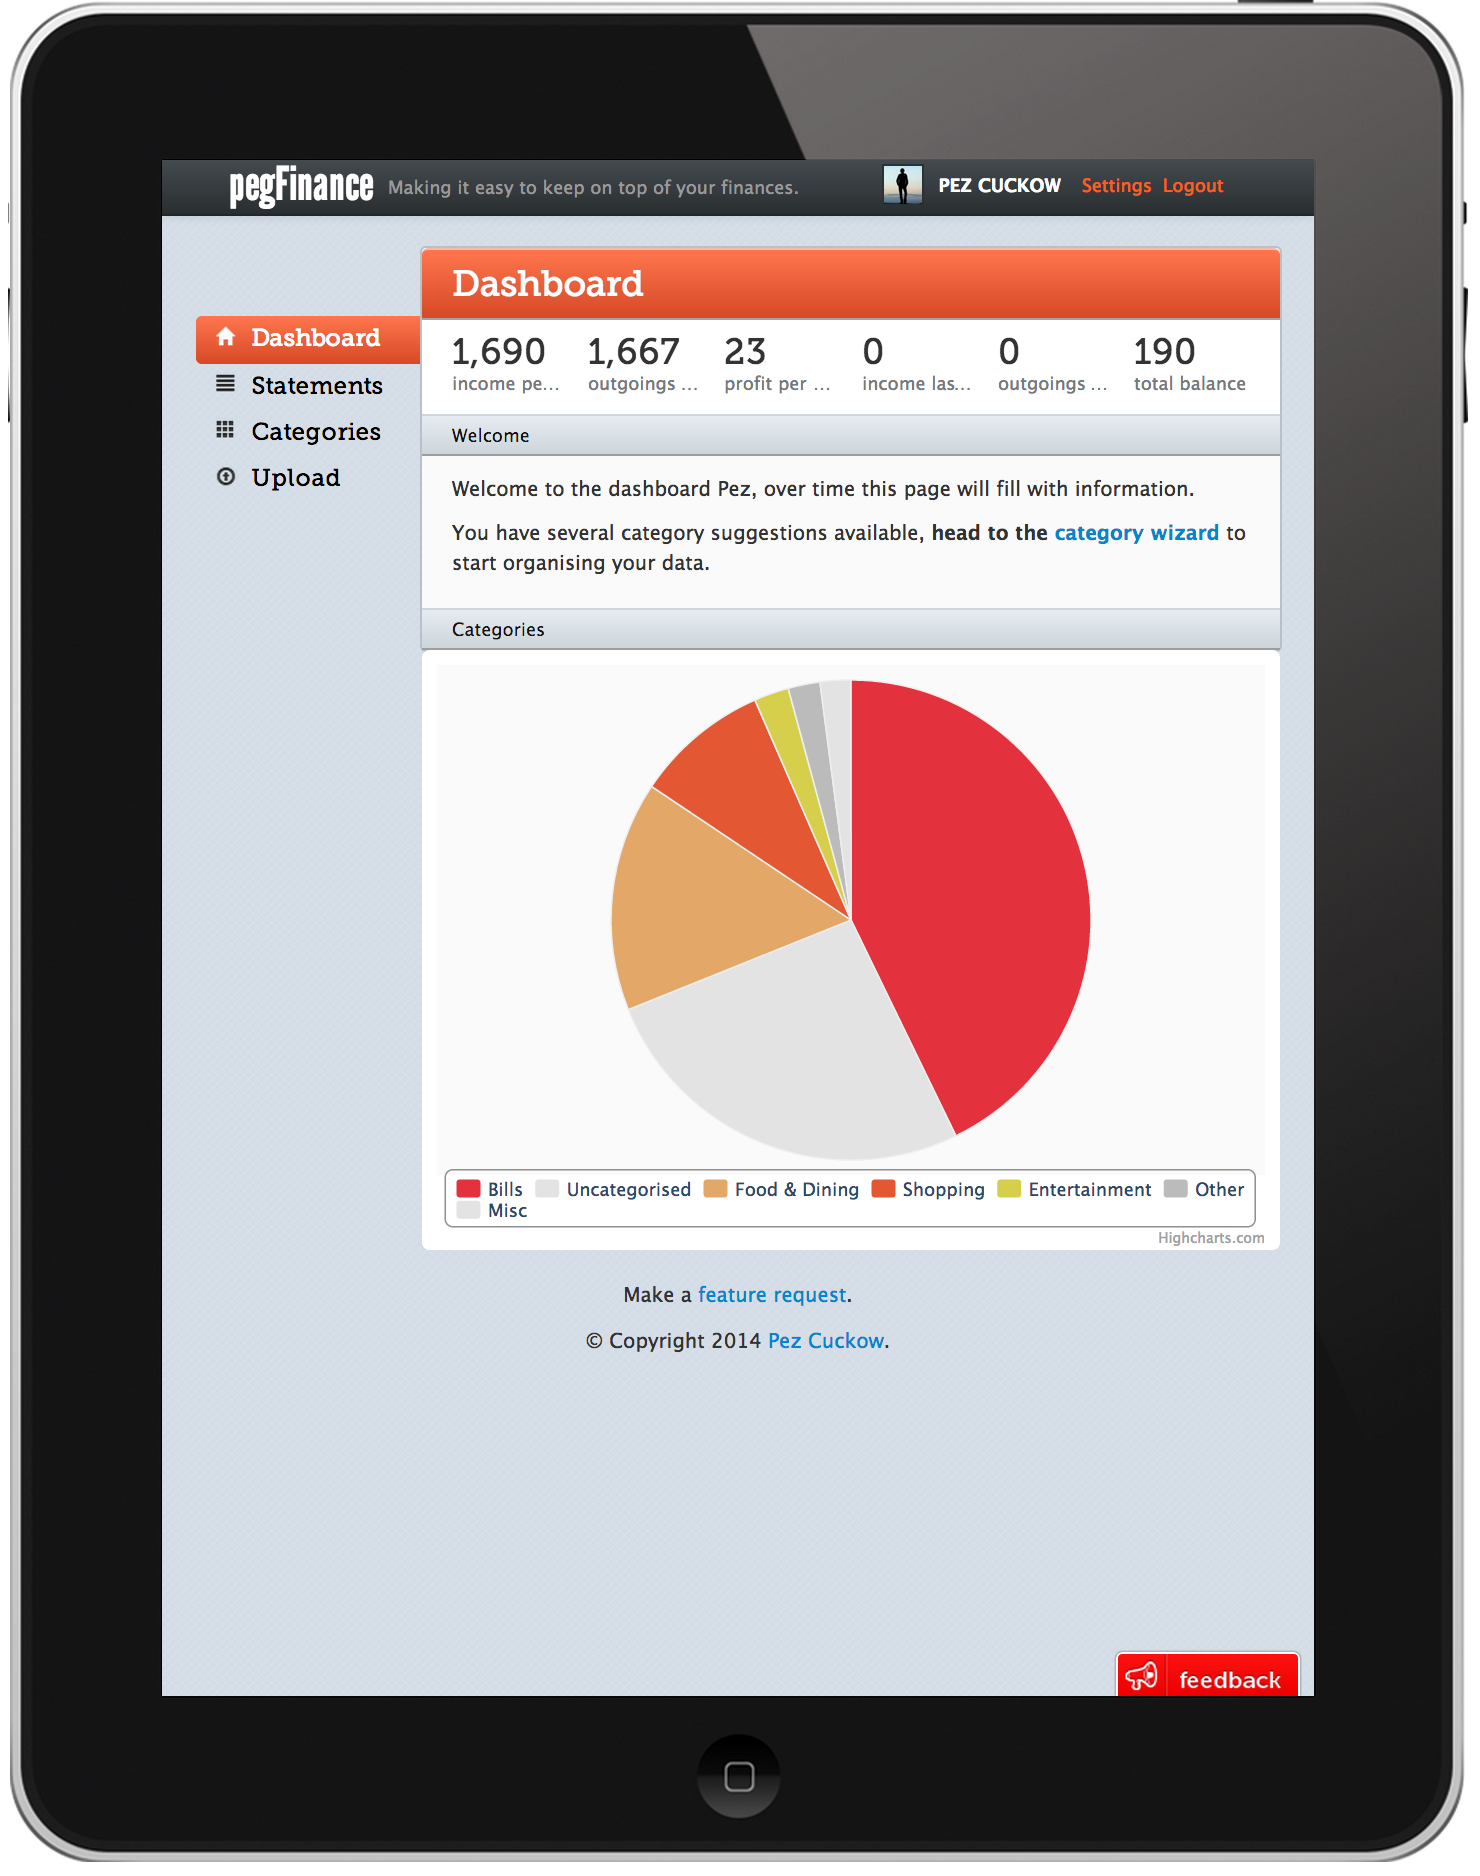
\includegraphics[width=0.5\textwidth]{screenshots/responsive/ipad-portrait}
    \caption{Layout on a tablet in portrait}
    \label{fig:responsive-ipad2}
\end{figure}

\begin{figure}[h]
    \centering
    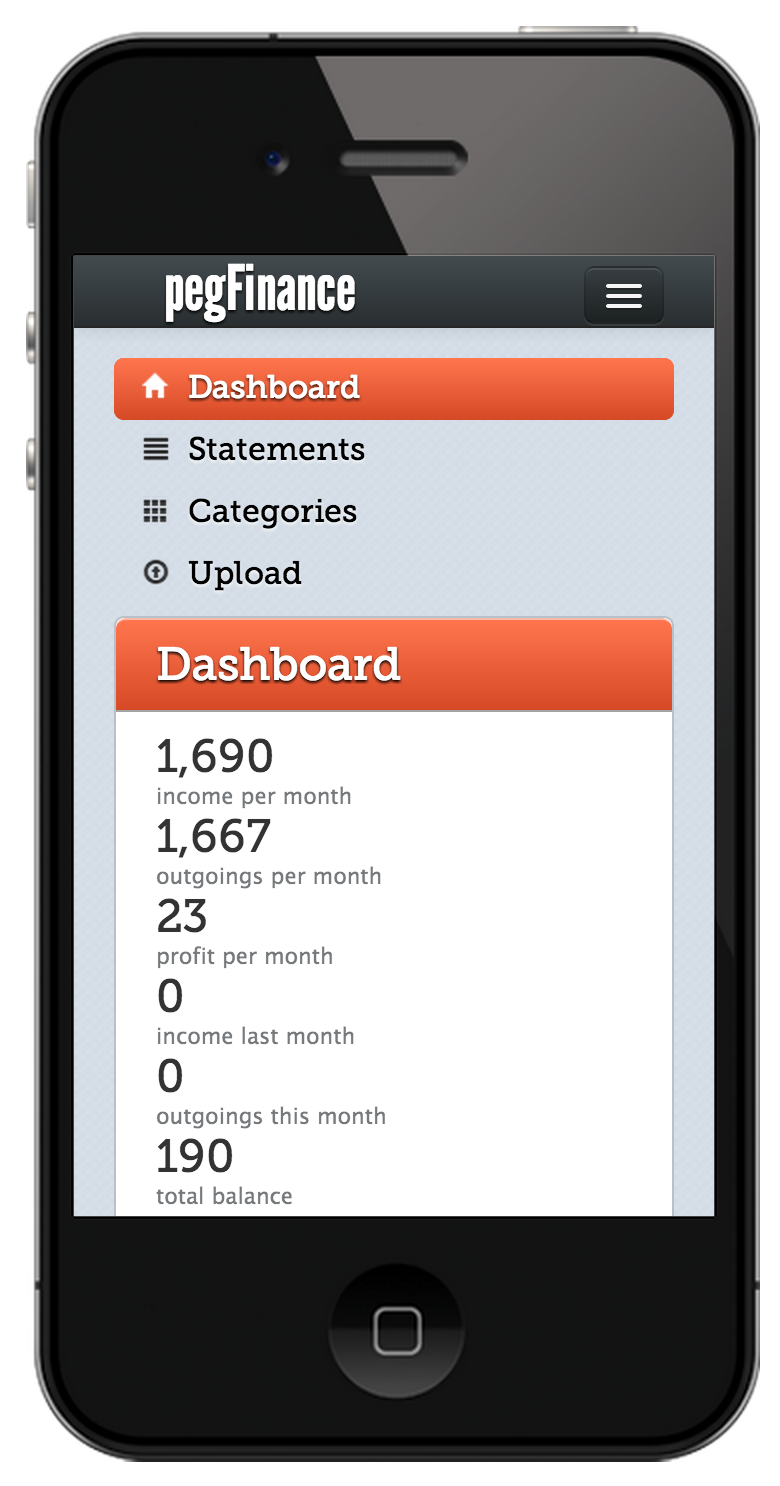
\includegraphics[width=0.5\textwidth]{screenshots/responsive/iphone-portrait}
    \caption{Layout on a smaller smartphone}
    \label{fig:responsive-iphone}
\end{figure}

%\section{Uploading a Statement}

%\section{Suggestion Engine}

%\section{Viewing Statements}

%\section{Prediction Overview}
\chapter{Testing and Evaluation}

\begin{comment}
Chapter 6: Testing and Evaluation
This chapter should give details of how the system designed and implemented by you was tested. The data and results obtained from this testing should be presented and consideration be given as to whether or not these results confirm that everything works correctly.

The analysis of test results is very important and some assessment of their significance and quality must be given. Likely sources of error and inaccuracy should be mentioned. Use graphs, bar charts and histograms where appropriate, remembering to label all axes and give scales. The analysis is often done badly, thus sacrificing marks.
\end{comment}

\section{Unit Tests}
\note{Not sure if this fits here!}

\section{Evaluation of the system}
\note{How did I check that it was working? Testing with personal data, users trying it and running tests of everything}

\missingfigure{Need figures representing accuracy, error, etc}

\section{User feedback}
\note{User surveys to check what they wanted}

\chapter{Conclusions}

\begin{comment}
Chapter 7: Conclusions
This can be a short chapter summarizing what you have achieved and what you have learned from the achievement. It is different from the abstract. The main results of your work should be highlighted with a critical appraisal of them indicating the extent to which the objectives outlined in Chapter 1 have been met. Exaggerated claims are counterproductive here. Recommendations for further activity are often included in this chapter.
\end{comment}

\section{Key Things Learnt}
\plan{How to do prediction, password entropy, other stuff}

\section{Does the system do what I set out to do?}
\plan{Does it make accurate predictions (summarise the evaluation section)}

\section{Further research}
\plan{Would like to classify users, would like to take into account global spending patterns}
% Gamification, global patterns

\subsection{Overfitting models}
\ref{section:overfittingmodels}

\plan{Include why having too many models is bad and explore those a bit}

\subsection{Using Learning to Select a Scaling Parameter}
\ref{section:learningscalingparameter}

\plan{How learning algorithms could be used to fit the weights even more (custom one for each user!)}

\section{Limitations of research?}
\plan{Limited set of testers, just students and friends, add more stuff and then go global.}



%% References
% There are a number of schemes for presenting references to the reader. Most publications are very strict about their presentation and, unfortunately, there is no unanimity of format across the range of relevant publications. The recommended method, used in IET and IEEE journals, is to identify each reference with a number located at the appropriate point of the text in square brackets, e.g. [42]. This is the recommended format for project reports in Computer Science. The list of references included in your report must give all the relevant information to enable the reader to find it.

% references
\printbibliography

% appendix
%TC:ignore 
\begin{appendices}

\chapter{Survey} \label{app:budgetsurvey}
Informal survey of 12 CS students in the third year lab. 

Questions:
\begin{enumerate}
\item Do you currently make a budget?
\item Do you stick to that budget?
\item Do you find your budget has a `positive' impact?
\end{enumerate}

% Booktabs require to add  to your document preamble
\begin{table}[h]
\centering
\caption{Survey Results}
\begin{tabular}{@{}llll@{}}
\toprule
       & \multicolumn{3}{l}{Question} \\ 
Answer & 1.       & 2.      & 3.      \\ \midrule
yes    & 5        & 1       & 3       \\
no     & 7        & 4       & 4       \\
n/a    & 0        & 7       & 5       \\ \bottomrule
\end{tabular}
\end{table}

\begin{comment}
Appendix A, B, C, etc.
These appendices can be very useful for giving detail that would otherwise disrupt the flow and readability of the report. They are given titles (e.g. "Appendix A: Example of the operation of the system") and bound in with the report. In general they are optional though, by convention, for a programming project, Appendix A often contains a non-trivial illustrative example of an input to the system and the corresponding output. For some projects, appendices may include tables of data. However, very long tables of data (more than about 10 pages) should be relegated to the Auxiliary Material, and not submitted as part of the Final Report. Program listings (apart from short code snippets) should likewise not be submitted as part of the Final Report.
\end{comment}

\chapter{Hashing Test} \label{app:hashingtest}

Implemented in PHP, test was run on a 2.7 Ghz Intel Core i7 with 16Gb of 1600Mhz DDR3 RAM.

\lstinputlisting[style=phpcolor]{code/passwordHashingTest.php}

\chapter{PHP Code} \todo{Needs a better name}

\begin{figure}
\lstinputlisting[style=phpcolor]{code/setTransactorMethod.php}
\caption{PHP Transaction->setTransactor(\$name) method source code}
\label{fig:settransactor}
\end{figure}

\begin{figure}
\lstset{style=phpcolor}
\begin{lstlisting}
if($dmy && $mdy || !$dmy && !$mdy)
    // ... prompt the user
else
    // ... continue conversion using the detected month format
\end{lstlisting}
\caption{Whether or not to prompt the user following month format detection}
\end{figure}
\chapter{Suggestion Wizard JSON}

The suggestion wizard is powered by AJAX, which makes JSON requests to a RESTful API on the backend, Fig. \ref{fig:json-examples} outlines an example set of communication.

\begin{figure}
    \begin{subfigure}[a]{\textwidth}
        \lstinputlisting[language=json]{code/suggestions.json}
        \caption{GET request sent \lstinline{/ajax/transactor/suggestions}}
    \end{subfigure}
    
    \begin{subfigure}[b]{\textwidth}
        \lstinputlisting[language=json]{code/map.json}
        \caption{POST request sent to \lstinline{/ajax/transactor/map}}
    \end{subfigure}
\end{figure}

\begin{figure}
    \ContinuedFloat   
    \begin{subfigure}[c]{\textwidth}
        \lstinputlisting[language=json]{code/create.json}
        \caption{POST request sent to \lstinline{/ajax/transactor/create}}
    \end{subfigure}
    
    \begin{subfigure}[d]{\textwidth}
        \lstinputlisting[language=json]{code/reply.json}
        \caption{Response from API following a successful map or create}
    \end{subfigure}    

    \caption{JSON encoded requests to the RESTful API}
    \label{fig:json-examples}
\end{figure}

\end{appendices}

%TC:endignore 